\chapter{Science of ice reservoirs}
\label{chap:science}

\cleanchapterquote{I could do with some scientific help from specialists. I am trying to collect data on how and
  where glaciers form best so that I can improve on them and people can use the technique elsewhere.
}{Chewang Norphel}{(Padmashree awardee, Inventor of ice terraces)}

Prior AIR volume estimates differ widely from each other, suffer from high uncertainties and are restricted to
the Ladakh region \cite{nusserSociohydrologyArtificialGlaciers2019, norphelSnowWaterHarvesting2015}. Moreover,
their dependence on the weather and construction strategy used limits their utility in estimating AIR volumes
across future winters or in new locations.  

Modelling is a powerful tool that allows estimation of AIR volumes across space and time. However, in-situ
measurements are required to tie these models to reality. The weather, water and volume measurements carried out
with an enormous input of manpower in the Indian Himalayas and the Swiss Alps provide a unique data basis for
AIR studies. The combination of measurements and modelling provides the key to understanding the influence of
the construction strategy and location on AIRs. 

In this chapter, we showcase the AIR datasets collected and develop a physically-based model that can estimate
their volume evolution. Mass and energy balance equations were used to estimate the quantity of ice, meltwater,
sublimation, and wastewater. Sensitivity and uncertainty analysis were performed to identify the most sensitive
parameters and the variance they caused. For calibration, we chose two AIRs built across the winter of 2020/21
in India and Switzerland, and validated the model on a Swiss AIR built during 2019/20. In a second step, the
model was extended to serve as a tool for recommending discharge rates and identifying favourable construction
locations worldwide.


\section{Study sites and data}

We chose the Swiss Alps and the Indian Himalayan mountain regions to collect the required datasets described
above. The study period starts when the fountain was first switched on (start date) and ends when the respective
AIR either melted or broke into several ice blocks (expiry date).  Each AIR dataset was abbreviated based on the
construction strategy used, prefix of the country code and the suffix of the year of its expiry date. The
construction strategies are distinguished based on whether they used fountain scheduling strategies to regulate
water supply. Those that did were codenamed automated construction strategy whereas the rest were codenamed
traditional construction strategy. All except one construction campaign used traditional construction
strategies. Therefore, traditional AIRs are referred to without explicitly specifying their construction
strategy henceforth.

In total, ? AIRs were studied in these two regions across four winters  However, only four AIRs located in
Guttannen, Switzerland and one in Gangles, India had complete weather, water and volume measurements. Therefore,
only these AIR datasets are used in the following analysis. The rest of the AIR datasets are described in the
Appendix \ref{sec:add_data} and are used in later Chapters to perform qualitative analysis.

\begin{figure}[htb]
  \centering
	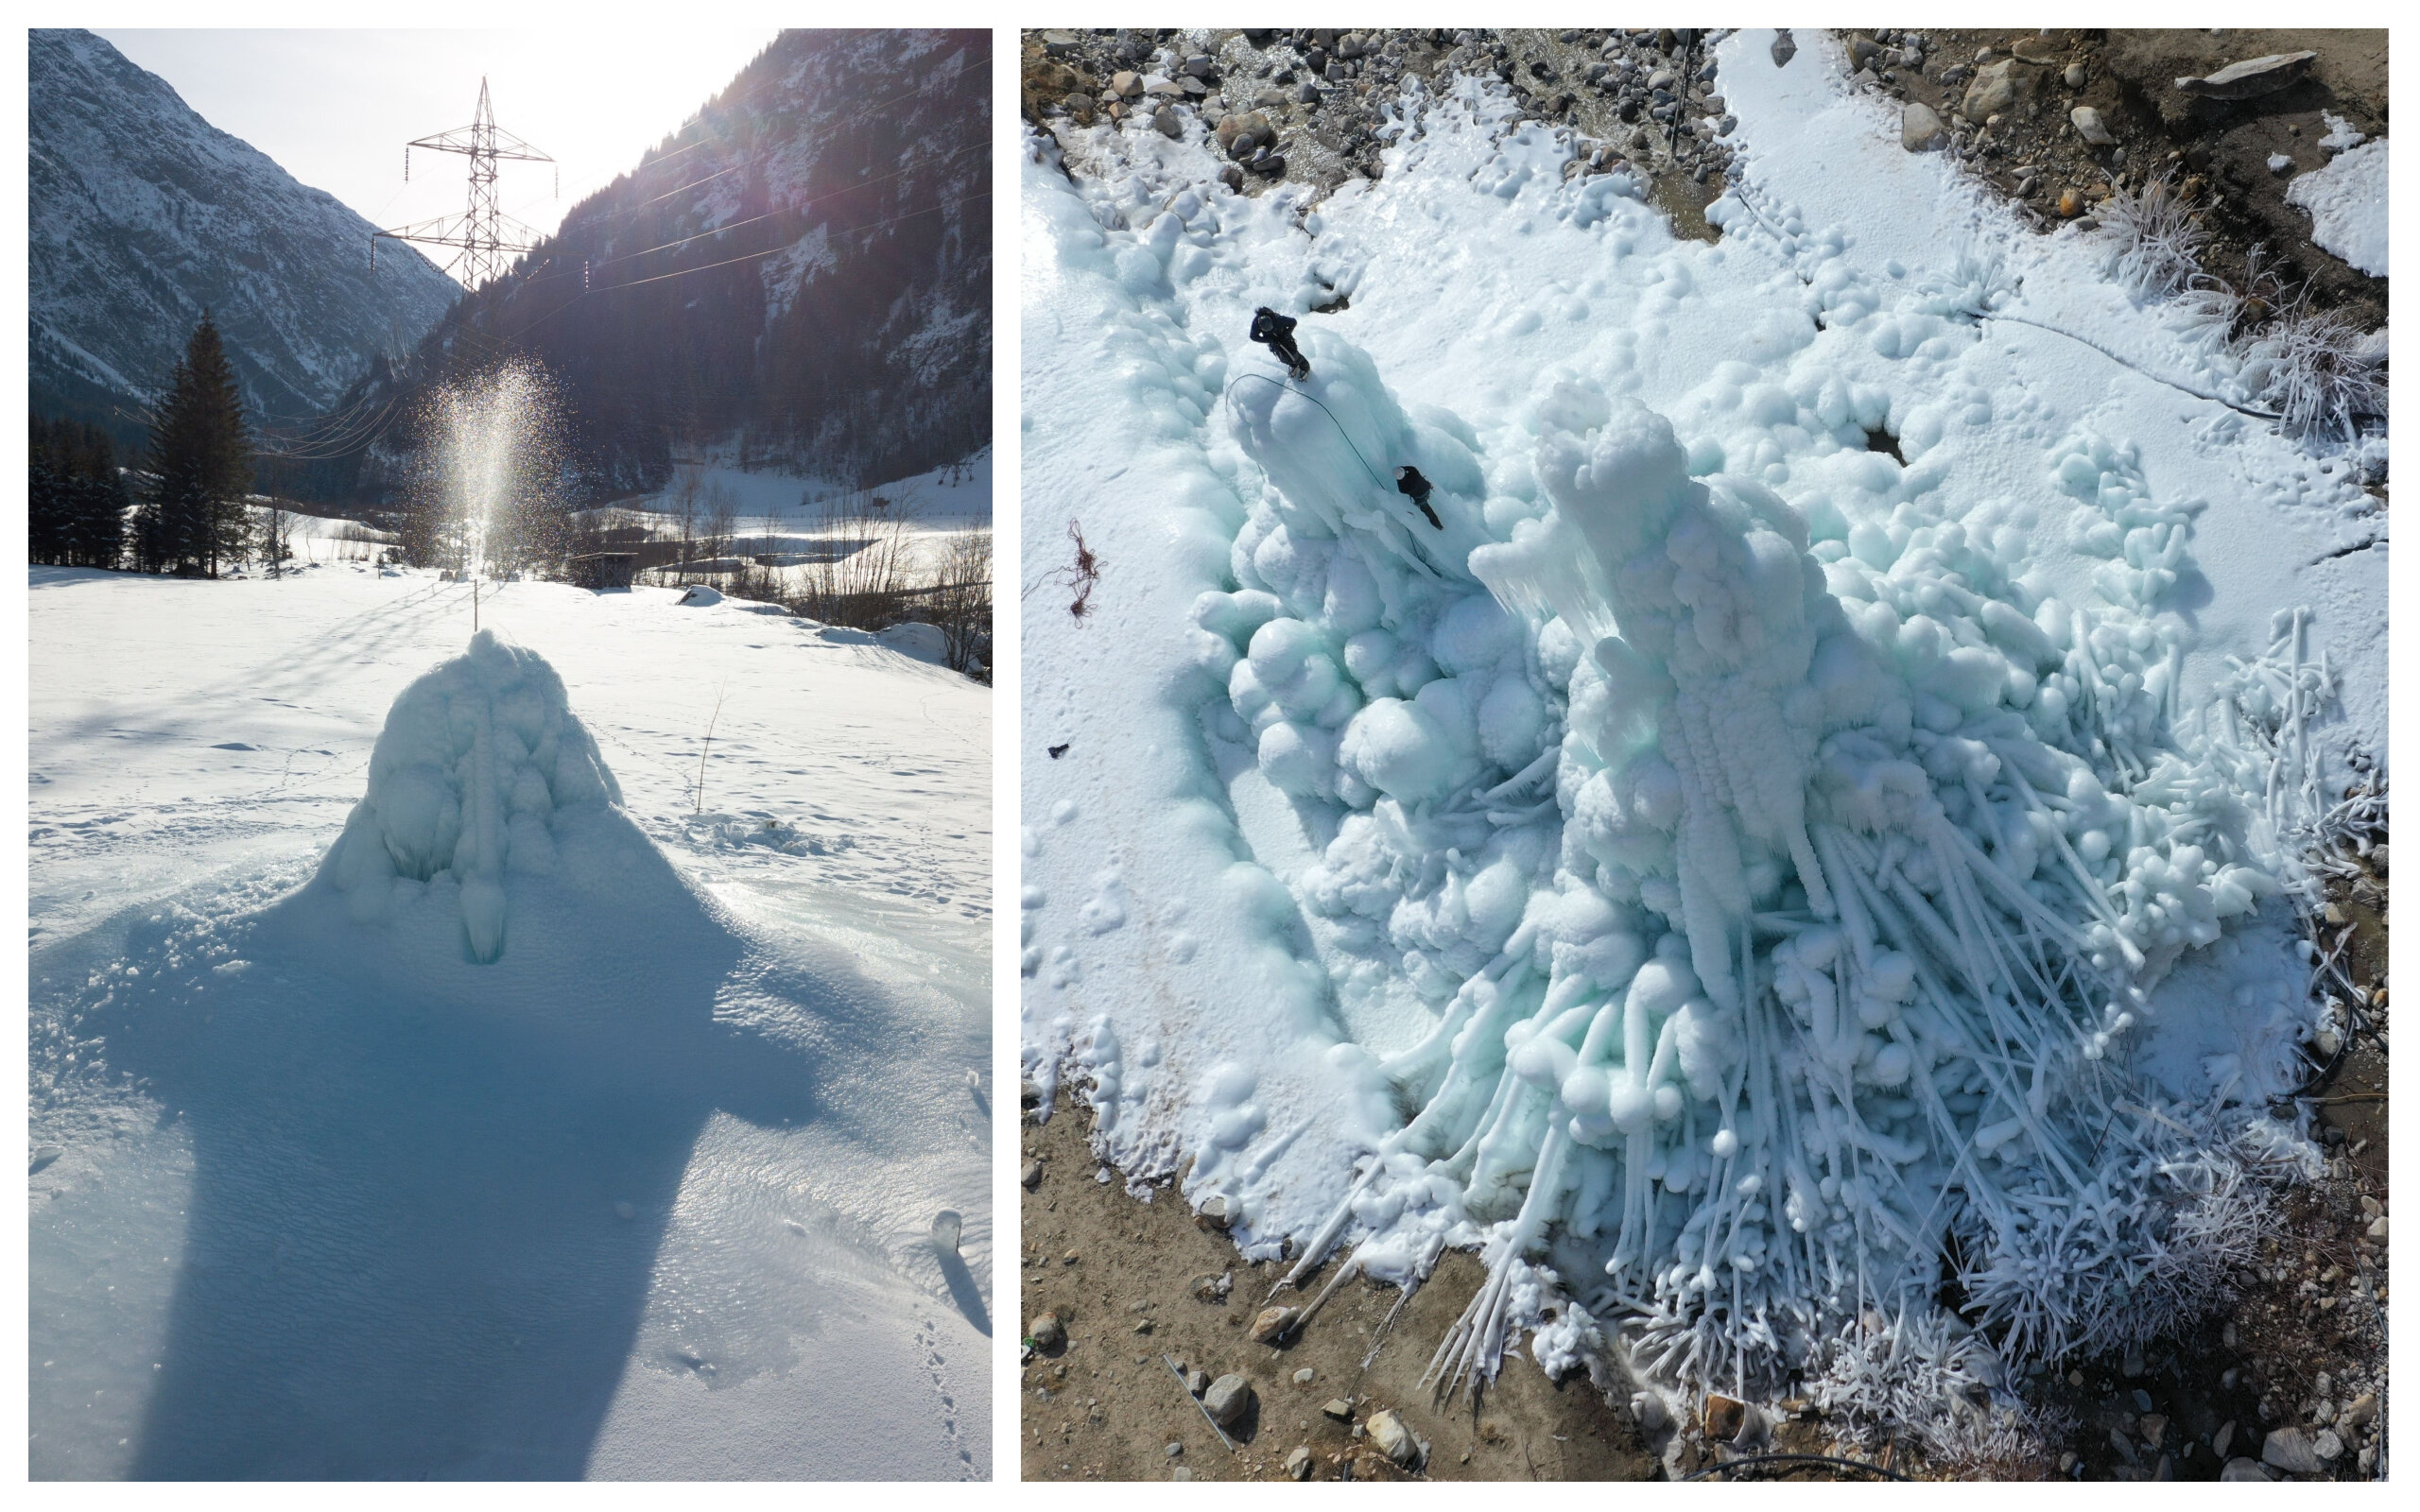
\includegraphics[width=12 cm]{figs/2AIRs.jpg}
  \caption{The Swiss and Indian AIRs were 5 $m$ and 13 $m$ tall on January 9 and March 3, 2021 respectively. Picture
credits: Daniel Bürki (left) and Thinles Norboo (right)}
\label{fig:2AIRs}
\end{figure}

\subsection{Swiss site}

The Guttannen site (46.66 $\degree$N, 8.29 $\degree$E) is situated in the Berne region, Switzerland and has an
altitude of 1047 $m$ a.s.l. In the winter (Oct-Apr), mean daily minimum and maximum air temperatures vary
between -13 and 15 $\degree C$. Clear skies are rare, averaging around 7 days during winter. Daily winter
precipitation can sometimes be as high as 100 $mm$. These values are based on 30 years of hourly historical
weather data measurements \citep{meteoblueClimateGuttannen2021}. Several AIRs were constructed by the Guttannen
Bewegt Association, the University of Fribourg and the Lucerne University of Applied Sciences and Arts during
the winters of 2020-22.

\subsection{Indian site}

The Gangles site (34.22 $\degree$N, 77.61 $\degree$E) is located around 20 km north of Leh city in the Ladakh
region, lying at 4025 $m$ a.s.l.. The mean annual temperature is $5.6 \, \degree C$, and the thermal range is
characterized by high seasonal variation. During January, the coldest month, the mean temperature drops to $-7.2
\, \degree C$. During August, the warmest month, the mean temperature rises to $17.5 \, \degree C$
\citep{nusserIrrigationDevelopmentUpper2012}. Because of the rain shadow effect of the Himalayan Range, the mean
annual precipitation in Leh totals less than 100 $mm$, and there is high interannual variability. Whereas the
average summer rainfall between July and September reaches 37.5 $mm$, the average winter precipitation between
January and March amounts to 27.3 $ mm$ and falls almost entirely as snow. AIRs were constructed here as part of
the Ice Stupa Competition by the Himalayan Institute of Alternatives, Ladakh (HIAL). 

\subsection{Meteorological data}

Air temperature, relative humidity, wind speed, pressure, longwave and global shortwave radiation are required
to calculate the surface energy balance of an AIR.  The resulting dataset highlights the difference in
meteorological influences driving ice volume evolution in the two study sites ( Table
\ref{tab:Observations}).

\begin{table}
  \centering
  \caption{Summary of the weather observations for AIRs built during the repective study period. 
The weather measurements are shown using their mean ($\mu$) and standard deviation ($\sigma$) during the study
period as $\mu \pm \sigma$. }

	\label{tab:Observations}
	\begin{tabular}{|lllll|}
    \hline
		\textbf{Name}               & \textbf{Symbol} & \textbf{IN21} & \textbf{CH21} & \textbf{Units}   \\ \hline
		Air temperature             & $T_a    $       & $0 \pm 7$     & $2 \pm 6$     & $\degree C$      \\
		Relative humidity           & $RH     $       & $35 \pm 20$   & $79 \pm 18$   & \%               \\
    Wind speed                  & $v_a        $   & $3 \pm 1$     & $2 \pm 2$     & $m/s$            \\
		Direct Shortwave            & $SW_{direct} $  & $246 \pm 333$ & $80 \pm 156$  & $W\,m^{-2}$      \\
		Diffuse Shortwave           & $SW_{diffuse}$  & $0 \pm 0$     & $58 \pm 87$   & $W\,m^{-2}$      \\
		Hourly Precipitation        & $ppt        $   & $0 \pm 0$     & $139 \pm 457$ & $mm$             \\
		Pressure                    & $p_a         $  & $623 \pm 3$   & $794 \pm 9$   & $hPa$            \\\hline
	\end{tabular}
\end{table}

\subsection{Fountain observations}

The fountain consists of a pipeline and a nozzle. The pipeline has three attributes, namely : discharge rate
($Q$), height ($h$) and water temperature ($T_F$). Discharge rate represents the discharge rate of the water in
the fountain pipeline. Height denotes the height of the fountain pipeline installed. Fountain water temperature
is the temperature of water droplets produced by the fountain.

The fountain nozzle has three characteristics, namely : the aperture diameter ($dia$) and pressure loss
($P_{nozzle}$) . Pressure loss denotes the loss of water head caused due to the fountain nozzle. Additionally,
the observed ice radius formed from the fountain water droplets is denoted as spray radius ($r_F$) (Fig.
\ref{fig:CH20_rad}). 

\begin{figure}[htb]
\centering
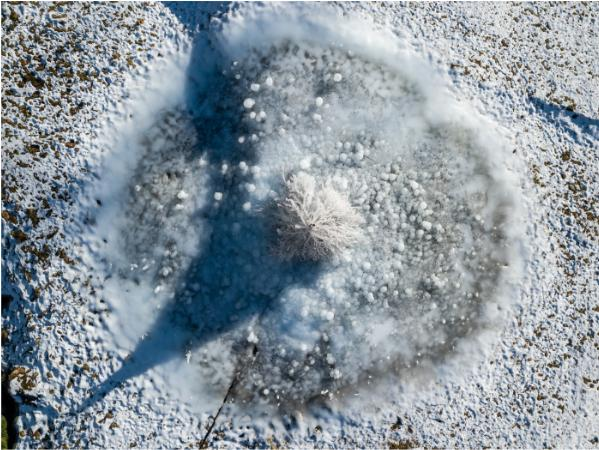
\includegraphics[width=\textwidth/2]{figs/CH20_sprayrad.jpg}
\caption{Spray radius of the CH20 AIR }
\label{fig:CH20_rad}
\end{figure}

\subsection{Drone flights}

\begin{table}
  \centering
  \caption{List of all the studied AIRs. The study period starts when the fountain was first switched on
  (denoted as Start Date) and ends when the respective AIR either melted or broke into several ice blocks
(denoted as Expiry Date). }
	\label{tab:AIRs}
	\begin{tabular}{|lllll|}
    \hline
		\textbf{Name}     & \textbf{Start Date} & \textbf{Expiry Date} & \textbf{No. of flights} & \textbf{Spray
    radius} \\ \hline
    Traditional CH20  & Jan 3 2020 & Apr 6 2020 & 2 & 7.7 $m$ \\
    Traditional CH21  & Nov 22 2020   & May 10 2021 & 8 & 6.9 $m$ \\
    Traditional IN21  & Jan 18 2021   & June 20 2021 & 6 & 10.2 $m$ \\
    Traditional CH22  & Dec 8 2021 & April 12 2022 & 8 & 4.1 $m$ \\
		Automated CH22  &  Dec 8 2021 & April 12 2022 & 6 & 4.8 $m$ \\ \hline
	\end{tabular}
\end{table}

Several photogrammetric surveys were conducted for each of the AIRs. The details of these surveys and the
methodology used to produce the corresponding outputs are explained in paper I. The digital elevation models
(DEMs) generated from the obtained imagery were analysed to document the ice radius, the surface area and the
volume of the ice structures. Ice radius measurements of drone flights which observed either an increase in AIR
circumference or volume were averaged to determine the fountain's spray radius. The number of drone surveys
conducted for each of the AIRs and the corresponding spray radius observed is shown in Table \ref{tab:AIRs}. 

\section{AIR Model}

A bulk energy and mass balance model is used to calculate the amounts of ice, meltwater, water vapour and
wastewater of the AIR. In each hourly time step, the model uses the AIR surface area, energy balance and mass
balance calculations to estimate its ice volume, surface temperature and wastewater as shown in Fig.
\ref{fig:schema}.

\begin{figure}
	\begin{center}
		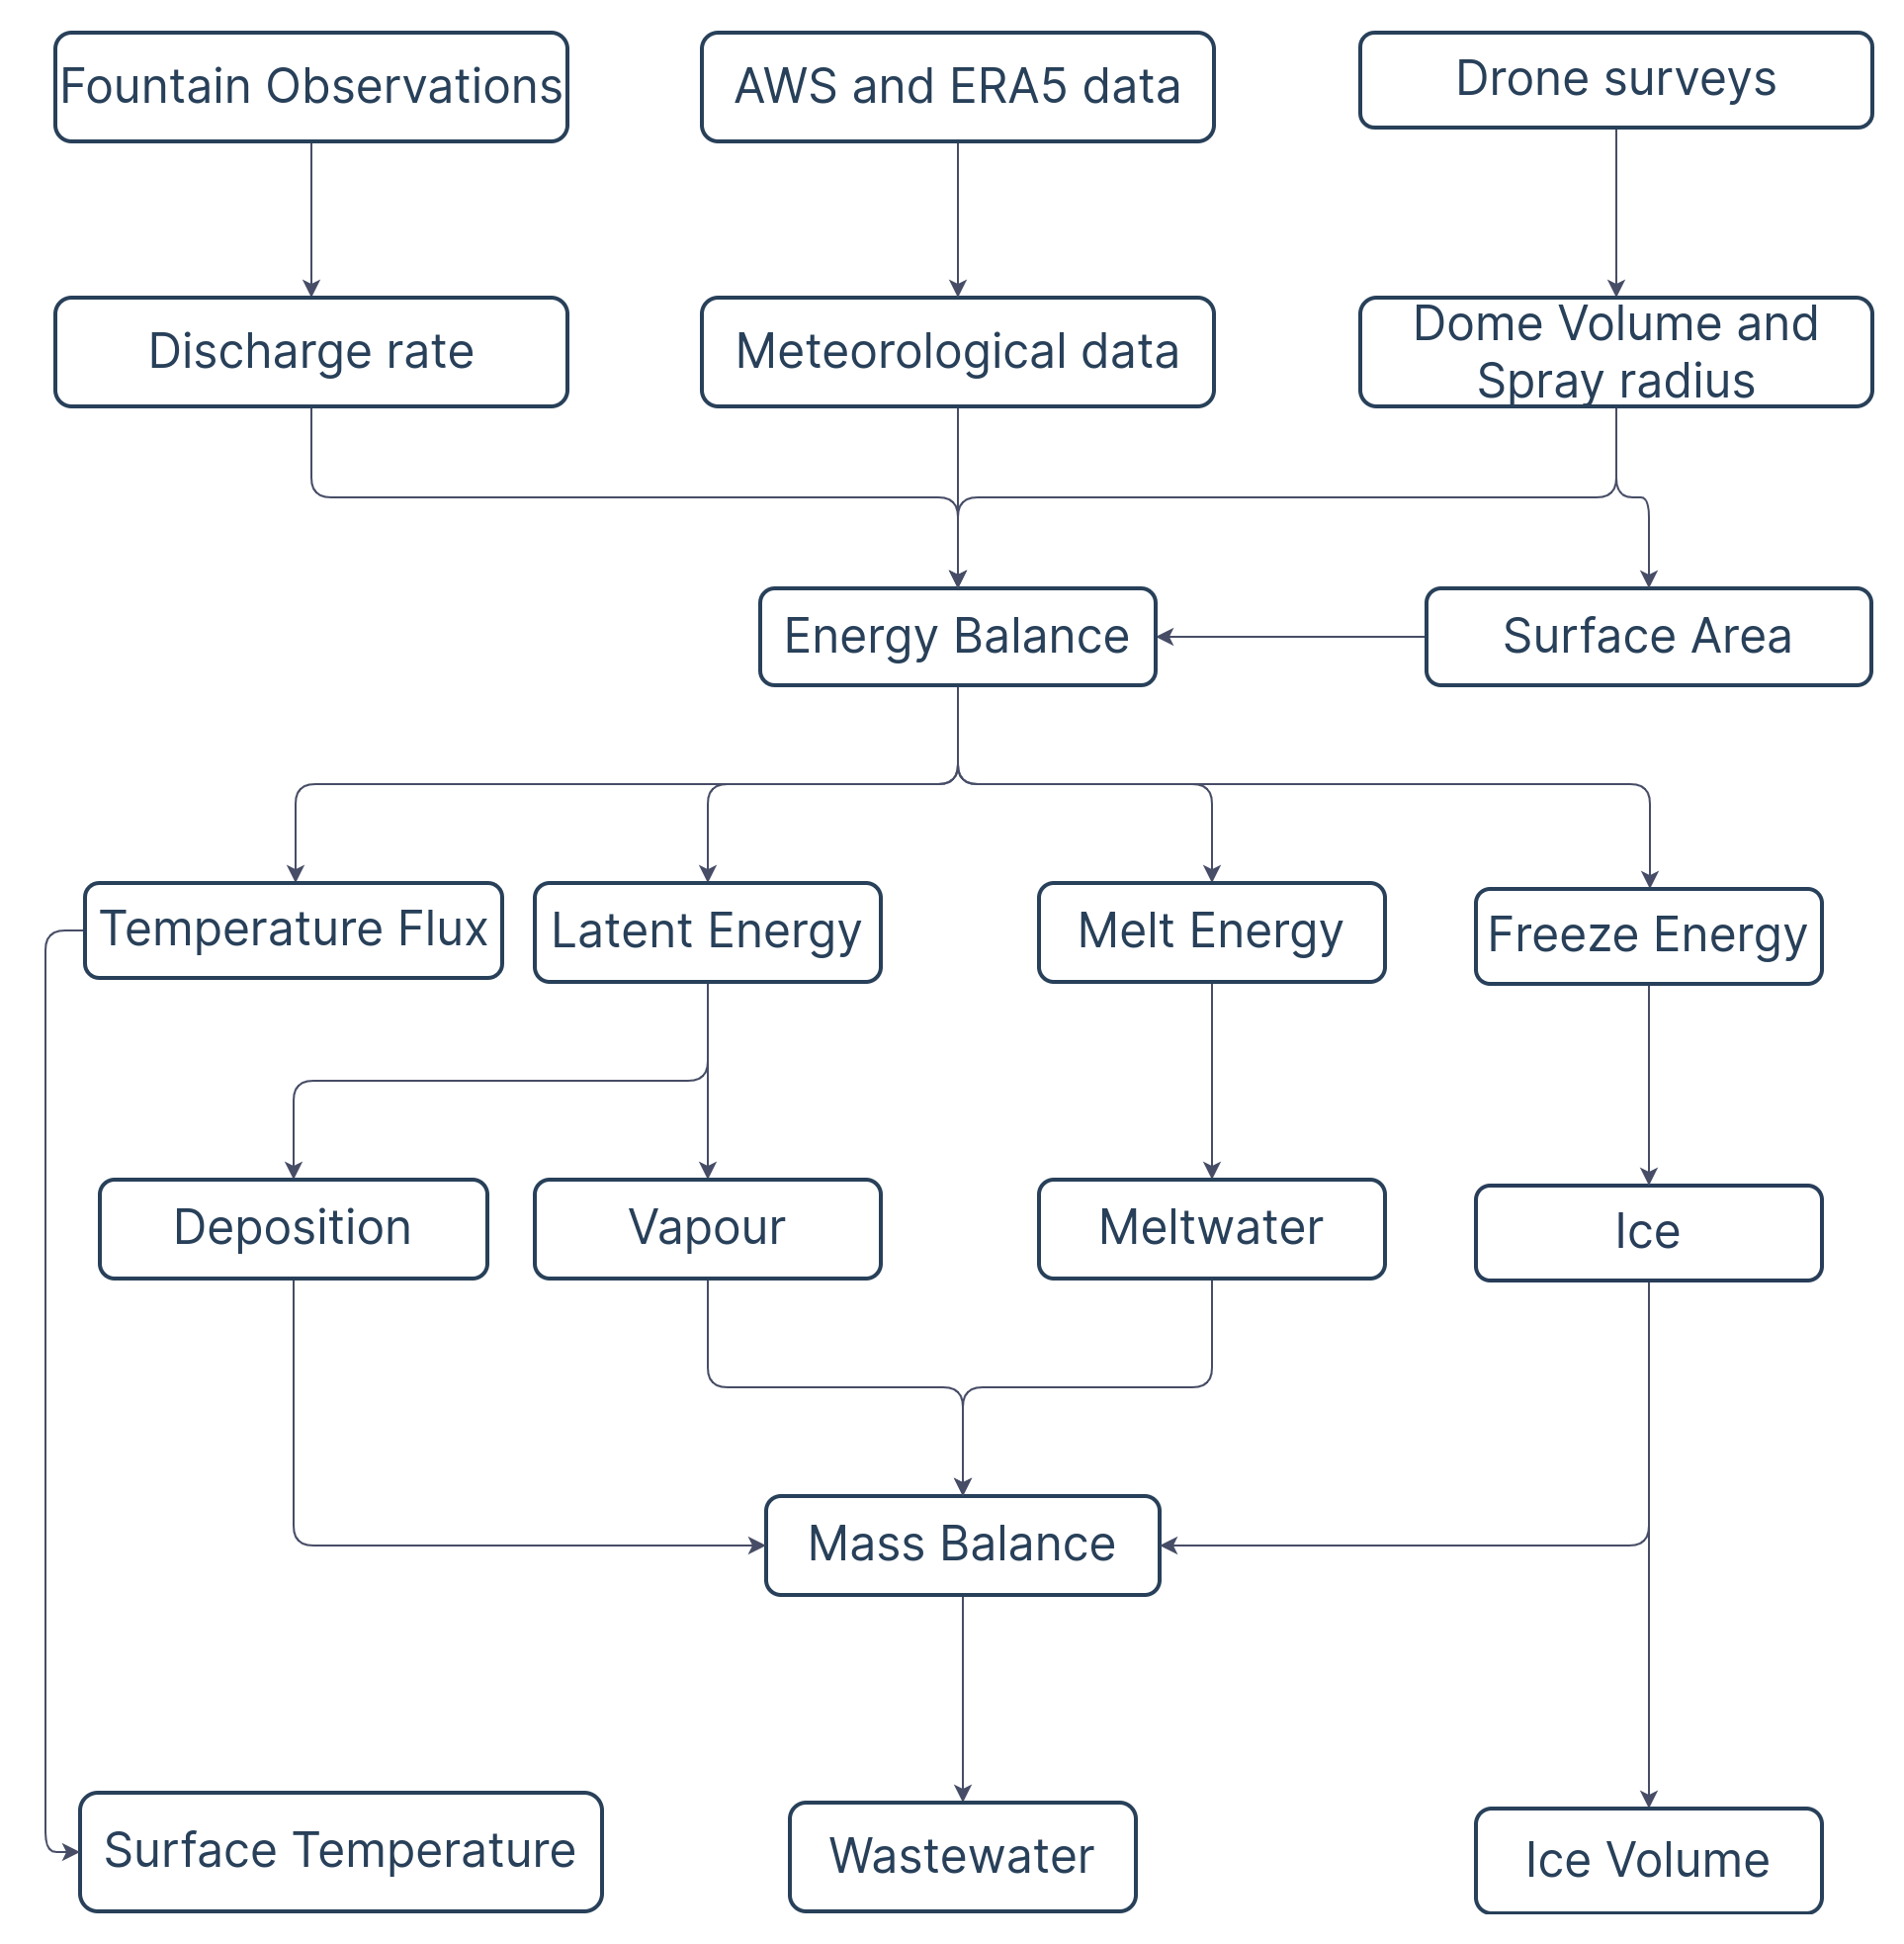
\includegraphics[width=10 cm]{figs/model_schematic.jpg}
	\end{center}
	\caption{Model schematic showing the workflow used in the model at every time step. }
	\label{fig:schema}
\end{figure}

\subsection{Surface area calculation} \label{sec:shape}

The model assumes the AIR shape to be a cone and assigns the following shape attributes:

\begin{subequations}
	\begin{align}
		\label{eq:A}
		A_{cone}^i & = \pi \cdot r_{cone}^i \cdot \sqrt{{(r_{cone}^i)}^2 + {(h_{cone}^i})^ 2} \\
		\label{eq:V}
		V_{cone}^i & = \pi/3 \cdot {(r_{cone}^i)}^2 \cdot h_{cone}^i                                         \\
		\label{eq:thickness}
		j_{cone}^i & =\frac{\Delta M_{ice}^i}{\rho_{water}* A_{cone}^i}
	\end{align}
\end{subequations}

where $i$ denotes the model time step, $r_{cone}^i$ is the radius; $h_{cone}^i$ is the height; $A_{cone}^i$ is
the surface area; $V_{cone}^i$ is the volume and $j_{cone}^i$ is the AIR surface normal thickness change as shown
in Fig. \ref{fig:shape}. $M_{ice}^i$ is the mass of the AIR and $\Delta M_{ice}^i = M_{ice}^{i-1} -
M_{ice}^{i-2}$. Henceforth, the equations used display the model time step superscript $i$ only if it is different
from the current time step.

AIR density can be defined as:

\begin{equation}
  \rho_{cone} = \frac{M_{F} + M_{dep} + M_{ppt}}{(M_{F} + M_{dep})/\rho_{ice} + M_{ppt}/\rho_{snow}}
\end{equation}

where $M_F$ is the cumulative mass of the fountain discharge; $M_{ppt}$ is the cumulative precipitation;
$M_{dep}$ is the cumulative accumulation through water vapour deposition; $\rho_{ice}$ is the ice density (917
$kg\,m^{-3}$) and $\rho_{snow}$ is the density of wet snow (300 $kg\,m^{-3}$) taken from
\cite{cuffeyPhysicsGlaciers2010} .

AIR volume can also be expressed as:

\begin{equation} V_{cone} =\frac{M_{ice}} {\rho_{cone}} \label{eq:V1} \end{equation}

The initial radius of the AIR is assumed to be $r_F$. The initial height $h_0$ depends on the dome volume
$V_{dome}$ used to construct the AIR as follows:

\begin{equation}
	h_{0} =  \Delta x + \frac{3 \cdot V_{dome}}{\pi \cdot (r_F)^2 }
	\label{eq:h0}
\end{equation}

where $\Delta x$ is the surface layer thickness (defined in Section \ref{sec:energy})

During the subsequent time steps, the dimensions of the AIR evolve assuming a uniform thickness change ($j_{cone}$)
across its surface area with an invariant slope $s_{cone} = \frac{h_{cone}}{r_{cone}}$ .  During these time
steps, the volume is parameterised using Eqn. \ref{eq:V} as:

\begin{equation} V_{cone} = \frac{\pi \cdot {(r_{cone})}^3
		\cdot s_{cone}}{3} \label{eq:V2} \end{equation}

We define the Icestupa boundary through its spray radius, i.e. we assume ice formation is negligible when $r_{cone} >
	r_{F}$. Combining Eqns. \ref{eq:V},  \ref{eq:V1}, \ref{eq:h0} and \ref{eq:V2}, the geometric evolution of the
Icestupa at each time step $i$ can be determined by considering the following rules:

\begin{equation} (r_{cone},\, h_{cone}) = \left\{ \begin{array}{ll} (r_F ,\, h_0)                                                                          & \textit{ if } i=0 \\
		(r_{cone}^{i-1},\, \frac{3 \cdot M_{ice}}{\pi \cdot \rho_{ice} \cdot {(r_{cone}^{i-1})}^2}) & \textit{ if }
		r_{cone}^{i-1} \geq r_{F} \textit{ and } \Delta M_{ice} > 0                                                     \\ (\frac{3 \cdot M_{ice}}{\pi \cdot \rho_{ice} \cdot s_{cone}})^{1/3} \cdot (1,\,  s_{cone}) &
		otherwise\end{array} \right.  \label{eq:A2} \end{equation}


\subsection{Energy balance calculation} \label{sec:energy}

\begin{figure}
	\begin{center}
		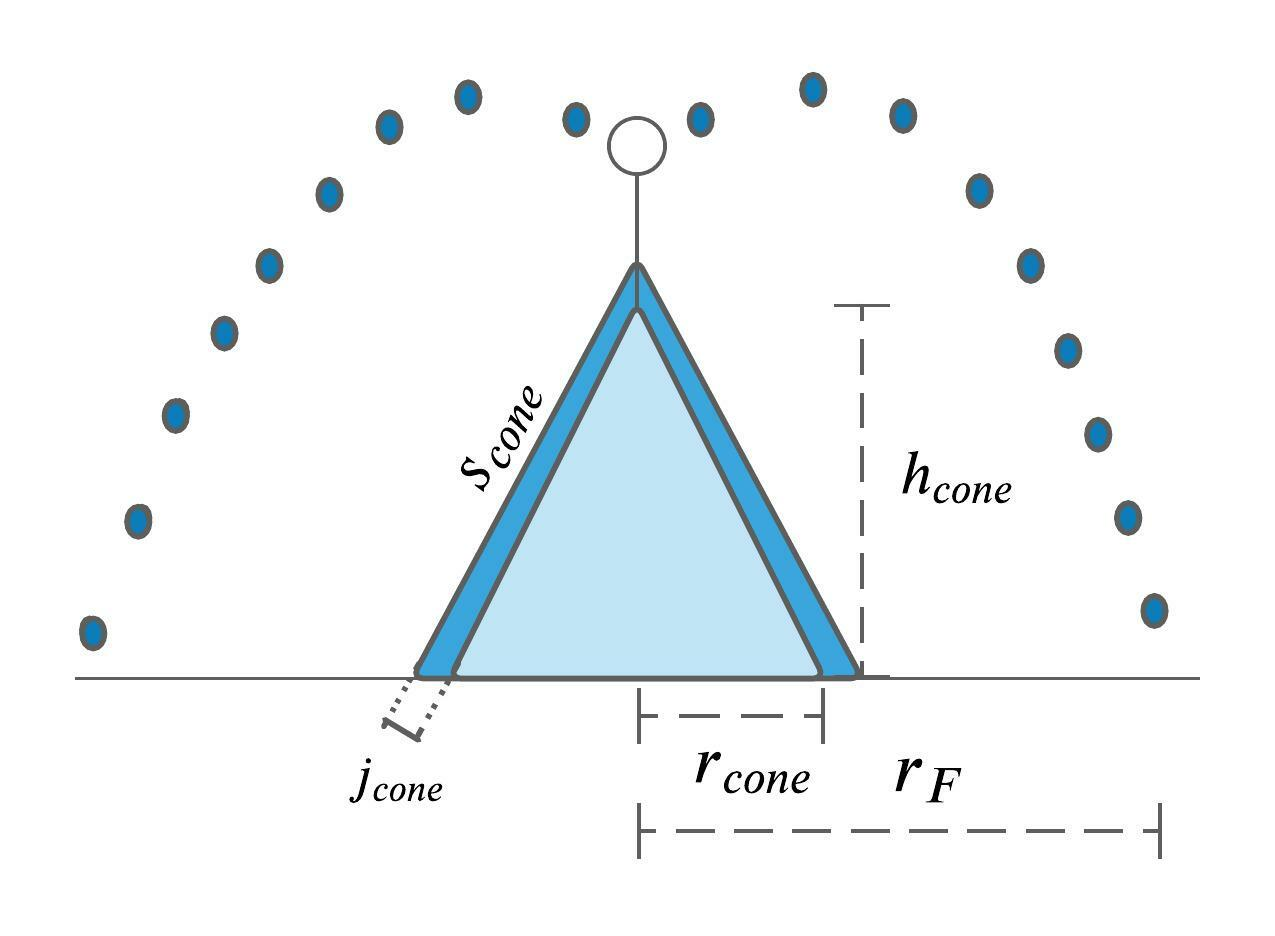
\includegraphics[width=10 cm]{figs/AIR_schematic.jpeg}
	\end{center}
	\caption{Shape variables of the AIR. $r_{cone}$ is the radius, $h_{cone}$ is the height, $j_{cone}$ is the
		thickness change and $s_{cone}$ is the slope of the ice cone. $r_F$ is the spray radius of the fountain.}
	\label{fig:shape}
\end{figure}

We approximate the energy balance at the surface of an AIR by a one-dimensional description of energy fluxes
into and out of a (thin) layer with thickness $\Delta x$:

\begin{equation}
  \rho_{cone} \cdot c_{ice} \cdot \frac{\Delta T}{\Delta t} \cdot \Delta x = q_{SW} + q_{LW} + q_{L} + q_{S} + q_{F}+ q_{R} + q_{G}
	\label{eqn:EB}
\end{equation}

Upward and downward fluxes relative to the ice surface are positive and negative, respectively. The first term
is the energy change of the surface layer, which can be translated into a phase change energy should phase
changes occur. $q_{SW}$ is the net shortwave radiation; $q_{LW}$ is the net longwave radiation; $q_{L}$ and
$q_{S}$ are the turbulent latent and sensible heat fluxes. $q_{F}$ and $q_{R}$ represent the heat exchange of
the fountain water droplets and rain droplets with the AIR ice surface respectively. $q_{G}$ represents ground
heat flux between the AIR surface and its interior.

The energy flux acts upon the AIR surface layer, which has an upper and lower boundary defined by the atmosphere
and the ice body of the AIR, respectively. Here, we define the surface temperature $T_{ice}$ to be the modelled
average temperature of the icestupa surface layer.

\subsubsection{Net Shortwave Radiation \texorpdfstring{$q_{SW}$}{Lg}} \label{sec:SW}

The net shortwave radiation $q_{SW}$ is computed as follows:

\begin{equation} q_{SW} = (1- \alpha)\cdot (SW_{direct} \cdot f_{cone} + SW_{diffuse}) \label{eqn:SW} \end{equation}

where $SW_{direct}$ and $SW_{diffuse}$ are the direct and diffuse shortwave radiation, $\alpha$ is the
modelled albedo and $f_{cone}$ is the area fraction of the ice structure exposed to the direct shortwave
radiation.

The albedo varies depending on the water source that formed the current AIR surface layer. During the fountain
runtime, the albedo assumes a constant value corresponding to ice albedo. However, after the fountain is
switched off, the albedo can reset to snow albedo during snowfall events and then decay back to ice albedo. We
use the scheme described in \cite{oerlemansYearRecordGlobal1998} to model this process. The scheme records the
decay of albedo with time after fresh snow is deposited on the surface. $\delta t$ records the number of time
steps after the last snowfall event. After snowfall, albedo changes over a time step, $\delta t$ , as

\begin{equation} \alpha=\alpha_{ice}+(\alpha_{snow}-\alpha_{ice}) \cdot e^{(-\delta t)/\tau} \label{eqn:alb}
\end{equation}

where $\alpha_{ice}$ is the bare ice albedo value (0.25), $\alpha_{snow}$ is the fresh snow albedo value (0.85)
and $\tau$ is a decay rate (16 $days$), which determines how fast the albedo of the ageing snow recedes back to
ice albedo. Discharge events decrease the decay rate by a factor of $\alpha_{ice}/\alpha_{snow}$. 

The solar area fraction $f_{cone}$ of the ice structure exposed to the direct shortwave radiation depends on the shape
considered. Using the solar elevation angle $\theta_{sun}$, the solar beam can be considered to have a vertical
component, impinging on the horizontal surface (semicircular base of the AIR), and a horizontal component
impinging on the vertical cross section (a triangle). The solar elevation angle $\theta_{sun}$ used is modelled
using the parametrisation proposed by \cite{woolfComputationSolarElevation1968}. Accordingly, $f_{cone}$ is determined as follows:

\begin{equation}
	\begin{split}
		f_{cone}& =\frac{(0.5 \cdot r_{cone} \cdot h_{cone}) \cdot cos \theta_{sun} +(\pi \cdot
			{(r_{cone})}^2/2) \cdot sin \theta_{sun} }{\pi \cdot r_{cone} \cdot ({(r_{cone})}^2+{(h_{cone})}^2)^{1/2}}\\
	\end{split}
	\label{eqn:f_{cone} }
\end{equation}

The diffuse shortwave radiation is assumed to impact the conical AIR surface uniformly.

\subsubsection{Net Longwave Radiation \texorpdfstring{$q_{LW}$}{Lg}} \label{sec:LW}

The net longwave radiation $q_{LW}$ is determined as follows:

\begin{equation}
	q_{LW}= LW_{in}-\sigma \cdot \epsilon_{ice} \cdot {(T_{ice}+ 273.15)}^4
	\label{eqn:LW}
\end{equation}

where $T_{ice}$ is the modelled surface temperature given in [$\degree C$],
$\sigma=5.67\cdot10^{-8}\,Jm^{-2}s^{-1}K^{-4}$ is the Stefan-Boltzmann constant, $LW_{in}$ denotes the incoming
longwave radiation and $\epsilon_{ice}$ is the corresponding emissivity value for the Icestupa surface (0.97).

The incoming longwave radiation $LW_{in}$ for the Indian site, where no direct measurements were available, is
determined as follows:

\begin{equation}
	LW_{in}=\sigma \cdot \epsilon_a \cdot {(T_a+ 273.15)}^4
	\label{eqn:LWin}
\end{equation}

here $T_a$ represents the measured air temperature and $\epsilon_a$ denotes the atmospheric emissivity. We
approximate the atmospheric emissivity $\epsilon_a$ using the equation suggested by \cite{brutsaertEvaporationAtmosphereTheory1982},
considering air temperature and vapor pressure (Eqn.  \ref{eqn:atm_e}). The vapor pressure of air over water and
ice was obtained using Eqn. \ref{eqn:vp}.  The expression defined in \cite{brutsaertDerivableFormulaLongwave1975} for clear skies
(first term in equation \ref{eqn:atm_e}) is extended with the correction for cloudy skies after
\cite{brutsaertEvaporationAtmosphereTheory1982} as follows:

\begin{equation}
	\epsilon_a=1.24 \cdot (\frac{p_{v,w}}{(T_a+273.15)})^{1/7}\cdot(1+0.22\cdot{cld}^2) \label{eqn:atm_e}
\end{equation}

with a cloudiness index $cld$, ranging from 0 for clear skies to 1 for complete overcast skies. For the Indian
site, we assume cloudiness to be negligible.

\subsubsection{Turbulent fluxes} \label{sec:Qs}

The turbulent sensible $q_{S}$ and latent heat $q_{L}$ fluxes are computed with the following expressions
proposed by \cite{garrattAtmosphericBoundaryLayer1992}:

\begin{equation}
	q_{S}=\mu_{cone}\cdot c_{a} \cdot \rho_{a} \cdot p_{a}/p_{0,a} \cdot \frac{\kappa^2 \cdot v_a \cdot
		(T_a-T_{ice})}{{(\ln{\frac{h_{AWS}}{z_{0}}})}^2}
	\label{eqn:qs}
\end{equation}

\begin{equation}
	q_{L}=\mu_{cone}\cdot 0.623 \cdot L_s \cdot \rho_{a}/p_{0,a} \cdot \frac{\kappa^2 \cdot
	v_a(p_{v,w}-p_{v,ice})}{{(\ln{\frac{h_{AWS}}{z_{0}}})}^2}
\end{equation}

where $h_{AWS}$ is the measurement height above the ground surface of the AWS (around $2\,m$ for all sites),
$v_a$ is the wind speed in [$m\,s^{-1}$], $c_a$ is the specific heat of air at constant pressure (1010 J
$kg^{-1} K^{-1}$), $\rho_{a}$ is the air density at standard sea level (1.29 $kg m^{-3}$), $p_{0,a}$ is the air
pressure at standard sea level (1013 $hPa$), $p_{a}$ is the measured air pressure, $\kappa$ is the von Karman
constant (0.4), $z_{0}$ is the surface roughness (3 $mm$) and $L_s$ is the heat of sublimation (2848
$kJ\,kg^{-1}$).  The vapor pressure of air with respect to water ($p_{v,w}$) and with respect to ice
($p_{v,ice}$) was obtained using the formulation given in \cite{huangSimpleAccurateFormula2018} :

\begin{equation}
	\begin{split}
		p_{v,w}&=e^{\frac{(34.494 - \frac{4924.99}{T_{a} + 237.1})}{(T_a + 105)^{1.57} \cdot 100}} \cdot \frac{RH}{100} \\
		p_{v,ice}&=e^{\frac{(43.494 - \frac{6545.89}{T_{ice} + 278})}{(T_{ice} + 868)^{2} \cdot 100}} \\
	\end{split} \label{eqn:vp}
\end{equation}

The dimensionless parameter $\mu_{cone}$ is an exposure parameter that deals with the fact that AIR has a rough
appearance and forms an obstacle to the wind regime. This factor accounts for the larger turbulent fluxes due to
the roughness of the surface \citep{oerlemansBriefCommunicationGrowth2021}, and is a function of the AIR slope
as follows:

\begin{equation}
	\mu_{cone} = 1 + \frac{s_{cone}}{2}
	\label{eqn:mu}
\end{equation}

A possible source of error is the fact that wind measurements from the horizontal plane at the AWS are used,
which might be different from those on a slope. However, without detailed datasets from the AIR surface, we
retain this assumption.

\subsubsection{Fountain discharge heat flux \texorpdfstring{$q_{F}$}{Lg} } \label{sec:heatflux}

The fountain water temperature $T_F$ is assumed to cool to 0 $\degree C$ after contact with the ice surface.
$T_F$ is equal to the measured source water temperature. But during time periods when the ambient temperature is
subzero, $T_F$ is assumed to be 0 $\degree C$. Thus, the heat flux caused by this process is:

\begin{equation}
	q_{F} = \left\{ \begin{array}{ll}
		\frac{ \Delta M_F \cdot c_{water} \cdot T_F}{\Delta t \cdot A_{cone}} & \textit{ if } T_{temp} > 0 \\
		0   & \textit{ otherwise}
	\end{array} \right.
\end{equation}

with $c_{water}$ as the specific heat of water (4186 J $kg^{-1} K^{-1}$).

\subsubsection{Rain heat flux \texorpdfstring{$q_{R}$}{Lg} }

The influence of rain events on the albedo and the energy balance was assumed to be similar to that of discharge
events. However, the water temperature of a rain event was assumed to equal to the air temeperature. Accordingly,
the heat flux generated due to a rain event was equal to:

\begin{equation}
  q_{R} = \frac{ \Delta M_{ppt} \cdot c_{water} \cdot T_a}{\Delta t \cdot A_{cone}}
	\label{eqn:qR}
\end{equation}

\subsubsection{Bulk Icestupa heat flux \texorpdfstring{$q_{G}$}{Lg}} \label{sec:Bulkflux}

The bulk Icestupa heat flux $q_{G}$ corresponds to the ground heat flux in normal soils and is caused by the
temperature gradient between the surface layer ($T_{ice}$) and the ice body ($T_{bulk}$). It is expressed by
using the heat conduction equation as follows:

\begin{equation} q_{G} = k_{ice} \cdot (T_{bulk}-T_{ice}^{i-1})/l_{cone} \label{eqn:qG}    \end{equation}

where $k_{ice}$ is the thermal conductivity of ice (2.123 $W\, m^{-1}\,K^{-1}$) , $T_{bulk}$ is the mean
temperature of the ice body within the icestupa and $l_{cone}$ is the average distance of any point in the
surface to any other point in the ice body. $T_{bulk}$ is initialised as 0 $\degree C$ and later determined from
Eqn. \ref{eqn:qG} as follows:

\begin{equation} T_{bulk}^{i+1} = T_{bulk} - (q_{G} \cdot A \cdot \Delta t)/(M_{ice} \cdot c_{ice}) \end{equation}

Since AIRs typically have conical shapes with $r_{cone} > h_{cone}$, we assume that the center of mass of the cone
body is near the base of the fountain. Thus, the distance of every point in the AIR surface layer from the cone
body's center of mass is between $h_{cone}$ and $r_{cone}$. Therefore, we calculate $q_{G}$ assuming $l_{cone} = (r_{cone} +
	h_{cone})/2$.

\subsubsection{Phase changes}\label{sec:phase}

In this section, the numerical procedures to model phase changes at the surface layer are explained. Let
$T_{temp}$ be the calculated surface temperature. Therefore, Eqn. \ref{eqn:EB} can be rewritten as:

$$q_{total} =\rho_{ice} \cdot c_{ice} \cdot \frac{(T_{temp}-T_{ice})}{\Delta t} \cdot \Delta x$$

where $q_{total}$ represents the total energy available to be redistributed. Even if the numerical heat transfer
solution produces temperatures which are $T_{temp}>0\, \degree C$, say from intense shortwave radiation, the ice
temperature must remain at $T_{temp} = 0\, \degree C$. The ‘‘excess’’ energy is used to drive the melting
process. Moreover, the energy input is used to melt the surface ice layer, and not to raise the surface
temperature to some unphysical value. Similarly, for freezing to occur, three conditions are required. Firstly,
fountain water is present ($\Delta M_{F} > 0 $) and secondly the calculated temperature of the ice, $T_{temp}$,
is below $0\, \degree C$. However, these two conditions are not sufficient as the latent heat turbulent fluxes
can only contribute to temperature fluctuations. Therefore, an additional condition, namely, $(q_{total}-q_{L})
< 0$, is required. Depending on the above conditions, the total energy $q_{total}$ can be redistributed
for the melting ($q_{melt}$), freezing ($q_{freeze}$) and surface temperature change ($q_{T}$) processes as
follows:

\begin{equation}
	q_{total} = \left\{ \begin{array}{ll}
		q_{freeze} + q_{T} & \textit{ if } \Delta M_{F} > 0 \textit{ and } T_{temp} < 0 \textit{ and }(q_{total}-q_{L}) < 0 \\
		q_{melt} + q_{T}   & \textit{ otherwise}
	\end{array} \right.
\end{equation}

Henceforth, time steps when the the total energy is redistributed to the freezing energy are called freezing
events and the rest of the time steps are called melting events.


During a freezing event, the AIR surface is assumed to warm to $0 \degree C$. The available energy
$(q_{total}-q_{L})$ is further increased due to this change in surface temperature represented by the energy
flux:

$$q_{0} = \frac{\rho_{ice} \cdot \Delta x \cdot c_{ice} \cdot T_{ice}^{i-1}}{\Delta t}$$

The available fountain discharge ($\Delta M_{F}$) may not be sufficient to utilize all the freezing energy. At such times, 
the additional freezing energy further cools down the surface temperature. Accordingly, the surface energy flux
distribution during a freezing event can be represented as:

\begin{equation}
	(q_{freeze}, q_{T}) = \left\{ \begin{array}{ll}
		(\frac{\Delta M_{F} \cdot L_f
		}{A_{cone} \cdot \Delta t}
		, q_{total}+\frac{\Delta M_{F} \cdot L_f
		}{A_{cone} \cdot \Delta t})          & \textit{ if  } \Delta M_{F} \textit{ insufficient }\\
		(q_{total}-q_{L}+q_{0}, q_{L}-q_{0}) & \textit{ otherwise }                                                                      \\
	\end{array} \right.
\end{equation}

If $T_{temp} > 0 \degree C$, then energy is reallocated from $q_{T}$ to $q_{melt}$ to maintain surface
temperature at melting point. The total energy flux distribution during a melting event can be represented as:

\begin{equation}
	(q_{melt}, q_{T}) = \left\{ \begin{array}{ll}
		(0, q_{total})
    & \textit{ if } T_{temp} \leq 0 \\
		(\frac{T_{temp} \cdot \rho_{ice} \cdot c_{ice} \cdot \Delta x}{\Delta t}, q_{total}-\frac{T_{temp} \cdot \rho_{ice} \cdot c_{ice} \cdot \Delta x}{\Delta t}  ) & \textit{ if } T_{temp} > 0
	\end{array} \right.
\end{equation}


\subsection{Mass balance calculation}

The mass balance equation for an AIR is represented as:

\begin{equation}
	\frac{\Delta M_{F} + \Delta M_{ppt} + \Delta M_{dep}}{\Delta t} = \frac{\Delta M_{ice} +\Delta M_{water} +
		\Delta M_{sub} + \Delta M_{waste}}{\Delta t}  \\
	\label{eq:MB}
\end{equation}

where $M_{F}$ is the cumulative mass of the fountain discharge; $M_{ppt}$ is the cumulative precipitation;  $M_{dep}$ is the cumulative
accumulation through water vapour deposition; $M_{ice}$ is the cumulative mass of ice; $M_{water}$ is the cumulative
mass of melt water; $M_{sub}$ represents the cumulative water vapor loss by sublimation and $M_{waste}$ represents the
fountain wastewater that did not interact with the AIR. The left hand side of equation \ref{eq:MB} represents the rate of
mass input and the right hand side represents the rate of mass output for an AIR.

Precipitation input is calculated as shown in equation \ref{eq:ppt} where $\rho_{w}$ is the density of water (1000
$kg\,m^{-3}$), $\Delta ppt/ \Delta t$ is the measured precipitation rate in [$m\,s^{-1}$] and $T_{ppt}$ is the temperature threshold
below which precipitation falls as snow. Here, snowfall events were identified using $T_{ppt}$ as $1 \degree C$. Snow
mass input is calculated by assuming a uniform deposition over the entire circular footprint of the AIR.

The latent heat flux is used to estimate either the evaporation and condensation processes or sublimation and deposition
processes as shown in equation \ref{eq:vap}. During the time steps at which the surface temperature is below 0 $\degree C$ only
sublimation and deposition can occur, but if the surface temperature reaches 0 $\degree C$, evaporation and condensation
can also occur. As the differentiation between evaporation and sublimation (and condensation and deposition) when the
air temperature reaches 0 $\degree C$ is challenging, we assume that negative (positive) latent heat fluxes correspond
only to sublimation (deposition), i.e. no evaporation (condensation) is calculated.

Since we have categorized every time step as a freezing or melting event, we can determine the melting/freezing
rates and the corresponding meltwater/ice quantities as shown in equations \ref{eq:m_freeze/melt}, \ref{eq:mwat}
and \ref{eq:mcone}. Having calculated all other mass components, the fountain wastewater generated every
time step can be calculated using Eqn. \ref{eq:MB}.

\begin{subequations}
	\begin{align}
		\frac{\Delta M_{F}}{\Delta t} & = \left\{ \begin{array}{ll} \frac{60}{\rho_w \cdot \Delta t} \cdot d_F
			 & \textit{ if fountain is on} \\ 0 & \textit{ otherwise } \\\end{array} \right.                                             \\
		\label{eq:ppt}
		\frac{\Delta M_{ppt}}{\Delta t}                                    & = \left\{ \begin{array}{ll} \pi \cdot
        {(r_{cone})}^2 \cdot
			\rho_{w}\cdot \frac {\Delta ppt}{\Delta t} & \textit{ if } T_{a} < T_{ppt} \\ 0 & \textit{ if } T_{a} \geq T_{ppt} \\\end{array} \right.                                             \\
		\label{eq:vap}
		(\frac{\Delta M_{dep}}{\Delta t}, \frac{\Delta M_{sub}}{\Delta t}) & = \left\{ \begin{array}{ll} \frac{q_{L}
			\cdot A_{cone}}{L_s}\cdot (1,0)  & \textit{ if } q_{L} \geq 0 \\ \frac{q_{L}
			\cdot A_{cone}}{L_s}\cdot (0,-1) & \textit{ if } q_{L} < 0    \\\end{array} \right.                                             \\
		\label{eq:mwat}
		\frac{\Delta M_{water}}{\Delta t}                                  & = \frac{q_{melt} \cdot A_{cone} }{L_f}                                                   \\
	  \label{eq:m_freeze/melt}
    \frac{\Delta M_{freeze/melt}}{\Delta t} & = \frac{q_{freeze/melt} \cdot A_{cone} }{L_f} \\
		\label{eq:mcone}
		\frac{\Delta M_{ice}}{\Delta t}                                    & = \frac{q_{freeze}\cdot A_{cone} }{L_f} + \frac{\Delta M_{ppt}}{\Delta t} + \frac{\Delta
			M_{dep}}{\Delta t}- \frac{\Delta M_{sub}}{\Delta t}- \frac{\Delta M_{water}}{\Delta t}
	\end{align}
\end{subequations}

Considering AIRs as water reservoirs, their net water loss can be defined as:

\begin{equation} \textit{Net water losses} = \frac{M_{waste}+M_{sub}}{(M_F+M_{ppt}+M_{dep})} \cdot 100 \end{equation}


\subsection{Uncertainty Quantification}

The uncertainty in the model of estimating ice volumes is caused by three sources, namely, model forcing
data, model hyperparameters and model parameters. Model forcing data can further be divided into weather and
fountain forcing data. Significant uncertainty exists in the weather forcing data, particularly for all the
radiation measurements ($SW_{direct}, SW_{diffuse}, LW_{in}$) since they were taken from ERA5 dataset or an AWS
far away from the construction sites. Since no other weather datasets exist for comparison, especially near the
IN21 AIR, we are not accounting for uncertainties related to meteorological forcing data in this analysis.
Uncertainty in the fountain forcing data arises due to only some fountain parameters listed in Table
\ref{tab:parameters}. Fountain runtime $t_F$ has no uncertainty for the Swiss AIRs because no interruptions
occured during the study period. However, significant uncertainty exists for the IN21 AIR , where the
interruptions due to pipeline freezing events happened overnight but this was ignored in this analysis. Fountain
spray radius $r_F$ was measured using the drone survey and therefore also doesn't contribute to model
uncertainty. The choice of mean discharge rate $d_F$ for both sites was just a best guess, based on few observations made by the
flowmeter. So we associate this parameter by a large uncertainty of $\pm \,50\, \%$. For the fountain water
temperature $T_F$, we assumed an upper bound of $3\, \degree C$ since it is unlikely for it to have been beyond
this range considering winter conditions at all the sites. The model structure introduces uncertainty through
the spatial and temporal hyperparameters $\Delta x$ and $\Delta t$. By definition, $\Delta x$ is directly
proportional to $\Delta t$. Therefore, we fix the temporal resolution of the model at hourly timesteps and only
investigate the uncertainty caused by $\Delta x$ here. Since the surface layer thickness for an AIR does not
resemble to any parameter in the glaciological literature, we attribute a wide range of values for it (from 1 cm
to 10 cm). The model parameters are henceforth called as weather parameters to distinguish them from the
fountain forcing parameters. These were fixed within a range based on literature values ( Table
\ref{tab:parameters}). 

The three types of uncertain parameters namely, model hyperparameters ($\Delta x$), fountain forcing parameters
($d_F, T_F$) and weather parameters ($\epsilon_{ice}, z_0, \alpha_{ice}, \alpha_{snow}, T_{ppt}, \tau$) are
denoted as $Q^M, Q^F$ and $Q^W$ henceforth. Together, these nine parameters cause a large uncertainty in the ice
volume estimates. In order to reduce this uncertainty, we perform a global sensitivity analysis with the net
water loss as our objective. The objective of this sensitivity analysis was to reduce the dimension of the
parameter space by calibrating the parameters with high total-order sensitivities ($S_{T_{j}} > 0.5$). The
methodology to determine $S_{T_{j}}$ is described in Appendix \ref{sec:uncertainpy}. These sensitive model
parameters were calibrated based on the root mean squared error (RMSE) between the drone surveys and the model
estimations of the ice volume. For this calibration procedure, all the other parameters were set to the median
value of their respective ranges defined in Table \ref{tab:parameters}.  The sensitivity analysis and
calibration were carried out with the drone surveys of CH21 and IN21 AIRs. 

The model uncertainty was quantified separately for the remaining parameters in $Q^M, Q^F$ and $Q^W$ using the
corresponding $90\, \%$ prediction interval $I^M, I^F$ and $I^W$. The $90\, \%$ prediction interval, $I^k$, gives us the
interval within which $90\,\%$ of the ice volume outcomes occur when all the parameters in $Q^k$ are varied
assuming each has an independent uniform probability density function. $5\,\%$ of the outcomes are above and
$5\,\%$ are below this interval. The methodology to obtain this is described in Appendix \ref{sec:uncertainpy}.

For validation, the calibrated model was tested with two datasets namely, the expiry date of all AIRs and the
drone surveys of CH20 AIR.

\begin{table}
  \caption{Free parameters in the model categorised as constant, derived, model hyperparameters, weather and
  fountain forcing parameters with their respective values/ranges.}
	\label{tab:parameters}
	\begin{tabular}{lllll}
		\toprule
		\textbf{Constant Parameters}                       & \textbf{Symbol} & \textbf{Value} &
    \textbf{Unit} & \textbf{Refs} \\
    Van Karman constant & $\kappa$      & 0.4        &dimensionless & \cite{cuffeyPhysicsGlaciers2010}              \\
    Stefan Boltzmann constant & $\sigma$ & $\num{5.67 e-8} $& $W\, m^{-2}\, K^{-4}$ & \cite{cuffeyPhysicsGlaciers2010}\\
    Air pressure at sea level & $p_{0,a}$ & 1013 & $hPa$  & \cite{molgAblationAssociatedEnergy2004}\\
    Density of water & $\rho_{w}$ & 1000 & $kg\, m^{-3}$    & \cite{cuffeyPhysicsGlaciers2010}\\
    Density of ice & $\rho_{ice}$ & 917 & $kg\, m^{-3}$ & \cite{cuffeyPhysicsGlaciers2010}\\
    Density of air & $\rho_{a}$ &  1.29 & $kg\, m^{-3}$   & \cite{molgAblationAssociatedEnergy2004}\\
    Specific heat of water & $c_{w}$ & 4186 & $J\, kg^{-1}\,\degree C^{-1}$  & \cite{cuffeyPhysicsGlaciers2010}\\
    Specific heat of ice & $c_{ice}$ & 2097 & $J\, kg^{-1}\,\degree C^{-1}$ & \cite{cuffeyPhysicsGlaciers2010}\\
    Specific heat of air & $c_{a}$ & 1010 & $J\, kg^{-1}\,\degree C^{-1}$ &
    \cite{molgAblationAssociatedEnergy2004}\\
    Thermal conductivity of ice & $k_{ice}$ & 2.123  & $W\, m^{-1}\, K^{-1}$ & \cite{bonalesThermalConductivityIce2017} \\
    Latent Heat of Sublimation & $L_{s}$ & \num{2.848e6}  & $J\, kg^{-1}$ &   \cite{cuffeyPhysicsGlaciers2010}\\
    Latent Heat of Fusion & $L_{f}$ & \num{3.34e5} & $J\, kg^{-1}$ & \cite{cuffeyPhysicsGlaciers2010}\\
    Gravitational acceleration & $g$ & 9.81 & $m\, s^{-2}$ &\cite{cuffeyPhysicsGlaciers2010}\\
    Weather station height & $h_{AWS}$ & 2 & $m$ & assumed \\
    Model timestep                            & $\Delta t$            & $3600$           & $s$ & assumed \\
    Fountain spray radius & $r_{F}$             &             & $m$& measured \\
    Fountain runtime & $t_{F}$             &             &  $hours$ & measured \\\midrule
		\textbf{Derived Parameters} & \textbf{Symbol} & \textbf{} & \textbf{Unit} & \textbf{Section} \\
    Radius of AIR & $r_{cone}$ &  & $m$ & \ref{sec:shape}\\
    Height of AIR & $h_{cone}$ &  & $m$ & \ref{sec:shape}\\
    Slope of AIR  & $s_{cone}$ &  & dimensionless & \ref{sec:shape}\\
    Thickness change of AIR  & $j_{cone}$ &  & $m$  & \ref{sec:shape}\\
    Atmospheric emissivity & $\epsilon_{a}$ & & dimensionless    & \ref{sec:LW}\\
    Cloudiness & $cld$ &  & dimensionless  & assumed\\
    Vapour pressure over water & $p_{v,w}$ &  & $hPa$  & \ref{sec:Qs}\\
    Vapour pressure over ice & $p_{v,ice}$ &  & $hPa$ & \ref{sec:Qs}\\
    Solar elevation angle & $\theta_{sun}$ &  & $\degree$ & \ref{sec:SW}\\
    Albedo & $\alpha$ &  & dimensionless & \ref{sec:SW}\\
    Solar area fraction& $f_{cone}$ &  & dimensionless & \ref{sec:SW}\\
    Ice body and surface distance & $l_{cone}$ &  & $m$  & \ref{sec:Bulkflux}\\
    AIR surface temperature & $T_{ice}$ &  & $\degree C$  & \ref{sec:Bulkflux}\\
    AIR bulk temperature & $T_{bulk}$ &  & $\degree C$  & \ref{sec:Bulkflux}\\\midrule
		\textbf{Model Hyperparameters} & \textbf{Symbol} & \textbf{Range} & \textbf{Unit} & \textbf{Refs} \\
    Surface layer thickness             & $\Delta x$            & $[\num{1e-2},\num{1e-1}]$           & $m$ & assumed
    \\\midrule
		\textbf{Weather Parameters} & \textbf{Symbol} & \textbf{Range} & \textbf{Unit} & \textbf{Refs} \\
    Ice Emissivity                      & $\epsilon_{ice}$      & $[0.95,0.99]$         & dimensionless & \cite{horiInsituMeasuredSpectral2006}             \\
    Surface Roughness                   & $z_0$                 & $[\num{1e-3},\num{5e-3}]$            & $m$  & \cite{brockMeasurementParameterizationAerodynamic2006}       \\
    Ice Albedo                          & $\alpha_{ice}$        & $[0.15,0.35]$         & dimensionless  &
    \cite{steinerModellingIcecliffBackwasting2015, zollesRobustUncertaintyAssessment2019}           \\
    Snow Albedo                         & $\alpha_{snow}$       & $[0.8,0.9]$        & dimensionless  & \cite{zollesRobustUncertaintyAssessment2019}              \\
    Precipitation Temperature threshold & $T_{ppt}$             & $[0,2]$            & $\degree C$& \cite{shichangResponseZhadangGlacier2010}  \\
    Albedo Decay Rate                   & $\tau$                & $[10,22]$           & $days$ &
    \cite{schmidtImportanceAccurateGlacier2017, oerlemansYearRecordGlobal1998}   \\\midrule
		\textbf{Fountain Forcing Parameters} & \textbf{Symbol} & \textbf{Range} & \textbf{Unit} & \textbf{Refs} \\
    Discharge rate & $d_{F}$             & $[0.5 \cdot d_{F},1.5 \cdot d_{F}]$            & $l/min$& assumed  \\
    Water temperature & $T_{F}$             & $[0,3]$            & $\degree C$  & assumed  \\\bottomrule
	\end{tabular}
\end{table}

\section{Model calibration, uncertainty and validation}

\subsection{Calibration of sensitive parameters}

The total-order sensitivities of all the nine parameters with respect to the net water loss objective are shown
in Fig. \ref{fig:param_hist} (a) . In total, the global sensitivity analysis required 1432 model runs to determine
these sensitivities for each site. The only sensitive parameter ($S_{T_{j}} > 0.5$) for both AIRs was the
surface layer thickness. The RMSE between the drone surveys and the model ice volume estimates for different
surface layer thickness are shown in Fig. \ref{fig:param_hist} (b). The optimum value of $\Delta x$ was found to
be 45 $mm$ and 65 $mm$ with an RMSE of 9 $m^3$ and 30 $m^3$ for CH21 and IN21 AIRs respectively.

\begin{figure}
	\centering
	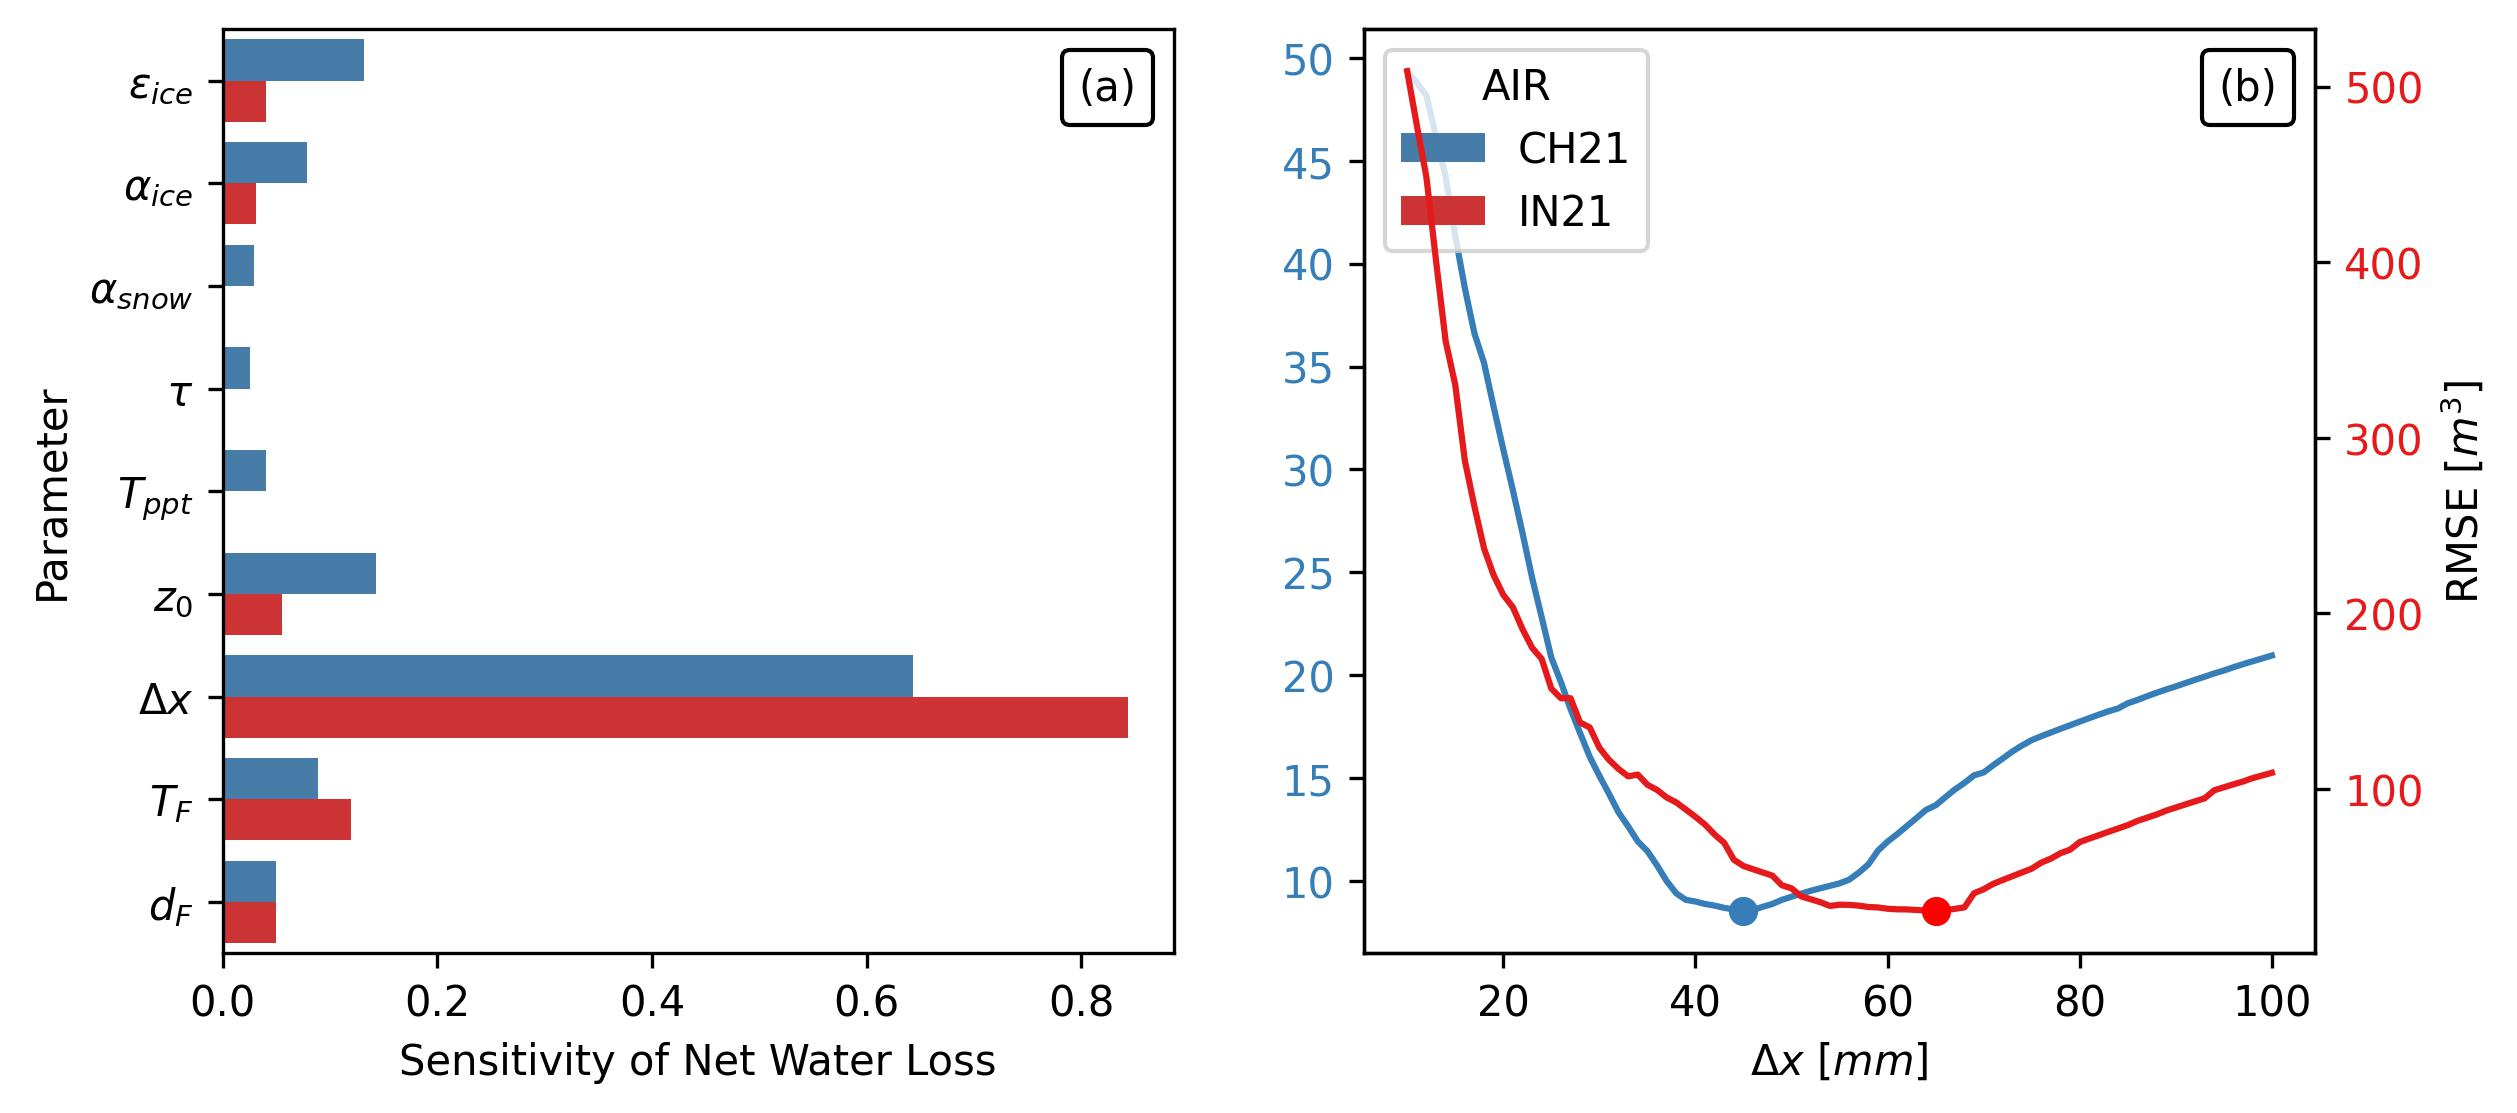
\includegraphics[width=\linewidth]{figs/model_calibration.jpg}
  \caption{(a) Total-order sensitivities of all the uncertain parameters of the model with net water loss as the
  objective. (b) The calibration of the sensitive parameter, $\Delta x$ with the RMSE between the drone and
model estimates of the ice volume. The dots denote the optimum values. The estimates from the Swiss and Indian
AIRs are denoted with blue and red colors respectively. }
	\label{fig:param_hist}
\end{figure}

\subsection{Weather and fountain forcing uncertainty quantification}

The uncertainty in the ice volume estimates caused by the weather and fountain forcing parameters are shown in
Fig. \ref{fig:results}. The ranges highlighted represent the corresponding $90\,\%$ prediction interval of the
ice volume estimates. Weather uncertainty determination required 422 simulations whereas fountain forcing
uncertainty determination required 32 simulations for each AIR. Since the results presented below differ
significantly during the fountain runtime, we divided the simulation duration of the AIR into accumulation and
ablation periods. The accumulation (ablation) period ends (starts) at the last fountain discharge event. 
 

The prediction interval of the weather and fountain forcing parameters behave differently during the
accumulation and ablation period for all AIRs. Prediction interval of the weather parameters increase
throughout the simulation period, but that of the fountain forcing parameters only increase during the
accumulation period. This is to be expected since the fountain forcing parameters directly affect the model
estimates only during the accumulation period. 

Weather uncertainty for the Indian site was low compared to the Swiss since precipitation and the associated
variation in albedo was negligible. At the end of the accumulation period, the Indian weather prediction
interval had a magnitude of  $73\,m^3$ which was 10 \% of the maximum simulated volume, whereas the magnitude of
the Swiss weather prediction interval was much higher (28 \% of the maximum simulated volume for the CH21 AIR).
This was expected since four out of the six uncertain Indian weather parameters were part of the albedo module. Among
all the weather parameters, surface roughness caused the most variance in both Indian and the Swiss ice
volume estimates.

Fountain forcing uncertainty for the Indian site was higher than its weather uncertainty (28 \% of the maximum
simulated volume at the end of the accumulation period). This was predominantly due to the uncertainty in the
fountain's water temperature. However, for the Swiss site, the prediction interval of the fountain forcing
parameters was similar to that of the weather parameters during the accumulation period. Since the mean fountain
discharge rate of the Indian location was eight times that of the Swiss, the uncertainty due to the fountain
forcing parameters was expected to be larger for the Indian location.

\subsection{Validation}

Model performance can be judged based on the ice volume left on the expiry date of all AIRs. In the case of CH21
AIR no ice volume was left whereas for CH20 AIR ice volume of 12 $m^3$ was left on the expiry date. For the IN21
AIR, the determination of the expiry date was not possible. In reality, the IN21 AIR was found to have
disintegrated into several ice blocks on 20th June, 2021. 

There was also one drone survey of the CH20 AIR volume for validation purposes. The RMSE of that observation
with the modelled volume was $19\, m^3$ which is 18 \% of the maximum simulated ice volume of CH20 AIR.

\begin{figure}
  \centering
	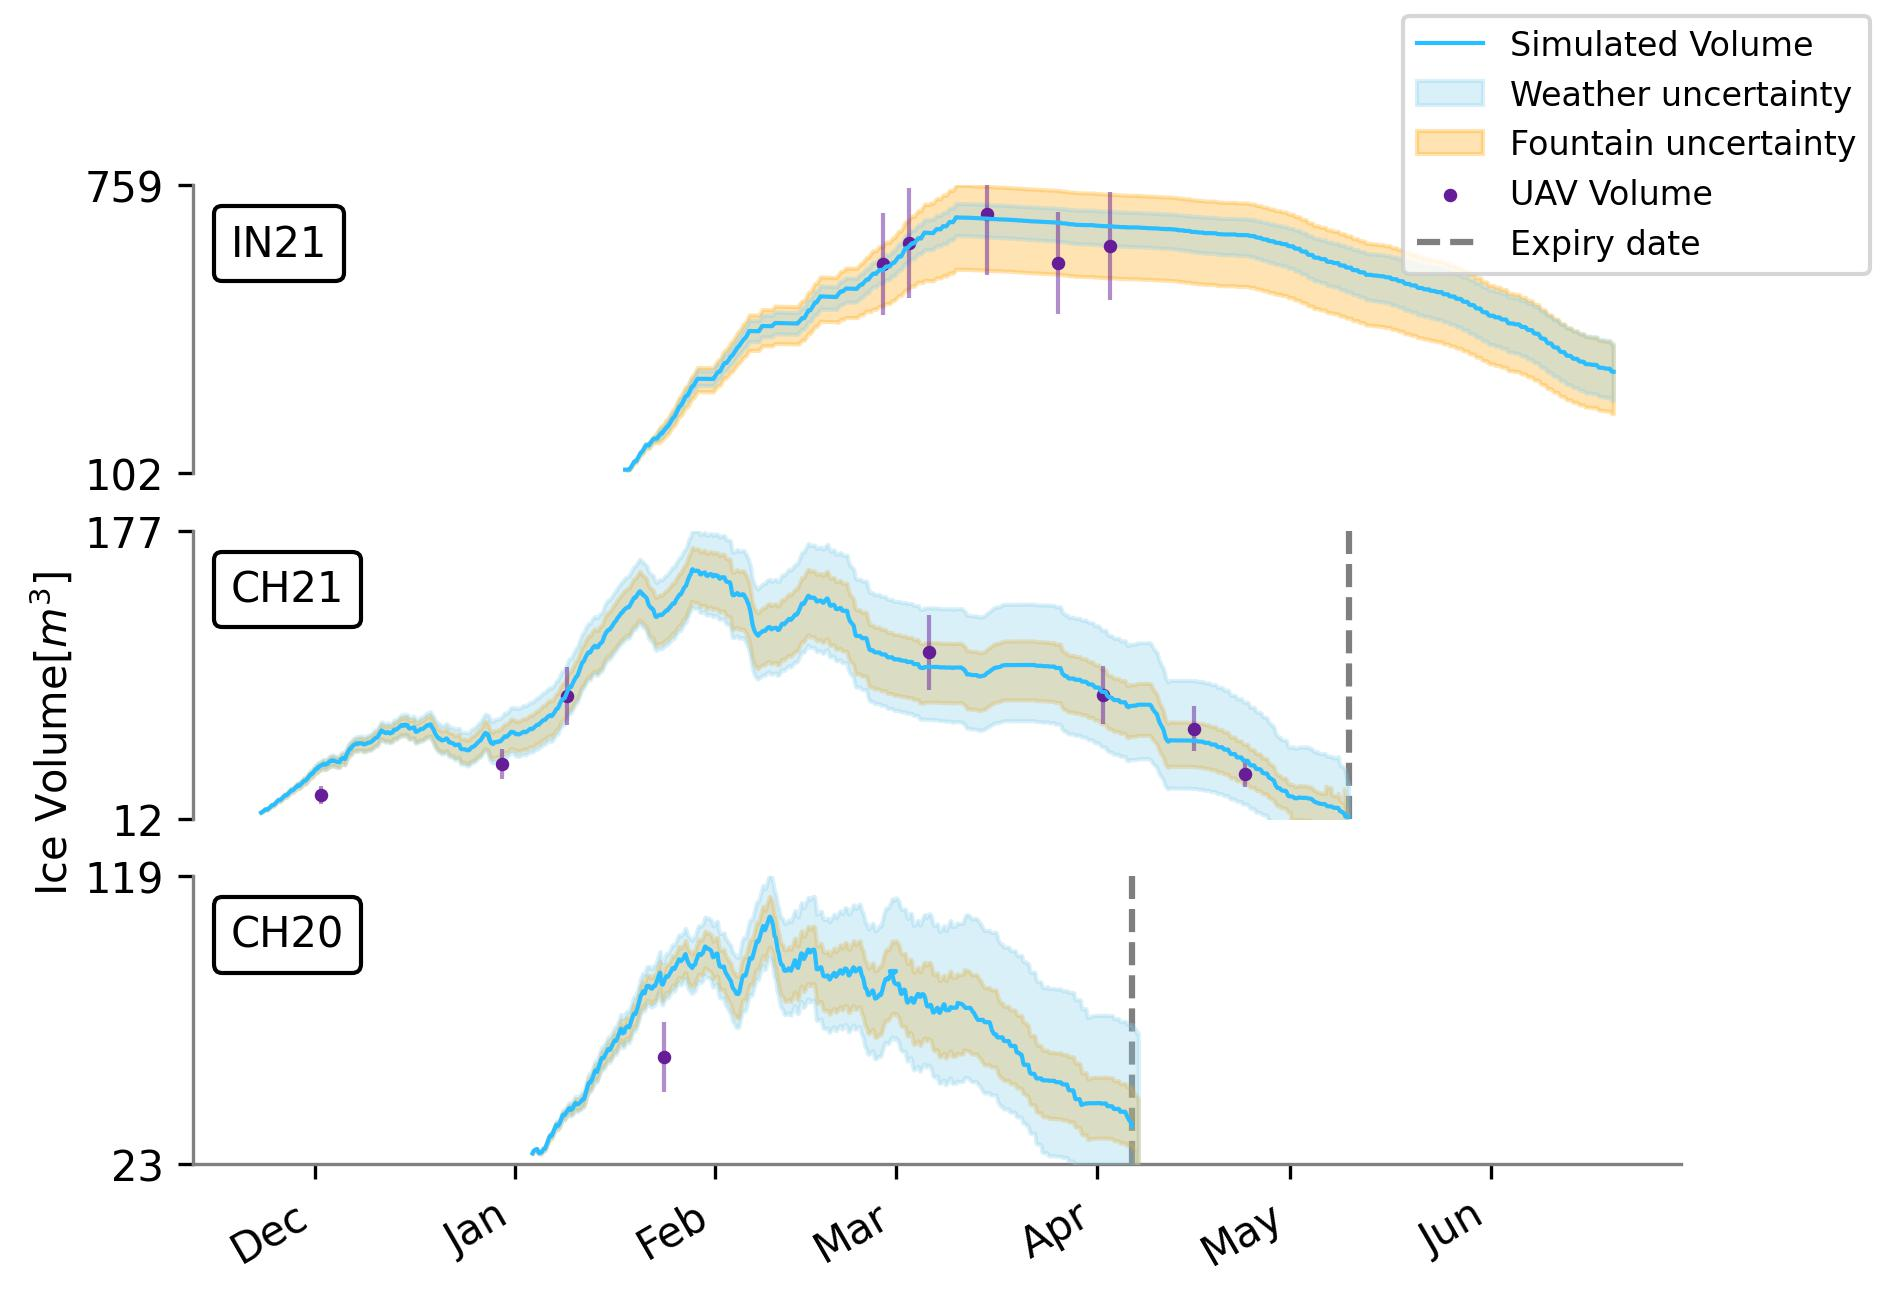
\includegraphics[width=\linewidth]{figs/model_validation.jpg}
	\caption{Simulated ice volume during the lifetime of the AIRs (blue curve). The shaded regions (light blue and
		orange) represent the 90\% prediction interval of the AIR ice volume caused by the variations in weather and
    fountain forcing parameters, respectively. Violet points indicate the drone ice volume observations.  The grey
  dashed line represents the observed expiry date for each AIR.  }
	\label{fig:results}
\end{figure}


\section{Model limitations and suggestions for improvement}

Model development is an art where subjective choices seek a balance between model simplicity and its accuracy.
Below we detail some of these choices and recommend strategies that shift this balance towards further model
accuracy.

\subsection{Quality and quantity of calibration and validation datasets}

The methodology used to acquire the radius, area and volume of AIRs ( Appendix \ref{sec:drone_method}) from
each drone survey has several drawbacks. The calibration and validation process used has an inherent temporal
and spatial bias due to the following subjective choices:

\begin{itemize}
  \item \textbf{The number of drone surveys}. For example, among the five surveys of IN21 AIR, most of them were
    conducted around early March when the AIR volume was near its maximum whereas the seven surveys of the CH21
    location were more evenly spaced out in comparison.

  \item \textbf{The weather conditions under which surveys were performed.} Particularly, precipitation events reduce DEM quality since
    they create uniform snow surfaces over AIRs. These surfaces dont have many identifiable features that can be
    used to extract the radius and area of the AIR.

\end{itemize}

Thus, the quality of AIR calibration and validation is severely limited by the high uncertainties attached with
the drone processing methodology.

This limitation can be overcome by extending the model validation set with daily AIR meltwater measurements.
However, the study site needs to satisfy two conditions in order to do this. First, the terrain of the site
needs to be waterproof and oriented so that most of the AIR runoff can be collected. Second, the chosen location
should not have high wind speeds, otherwise a significant fraction of AIR wastewater would be dispersed in the
air.

\subsection{Turbulent heat flux parametrization}

The method used to calculate turbulent heat fluxes by \citet{garrattAtmosphericBoundaryLayer1992} assumes that
these fluxes are acting over a uniform planar surface. This leads us to use the exposure/roughness parameter
$\mu$ as a correction factor. However, equation \ref{eqn:mu} about $\mu$ is no more than an educated guess. It
is hard to base estimates of this parameter on information in the literature. Many studies have been carried out
on the effect of obstacles on atmospheric boundary layer flow (e.g. trees), but always in an ensemble setting,
looking at the bulk effect of an ensemble of obstacles. We deal with a case of a single obstacle in open
terrain, and we are confident that the roughness of the surface and the exposure will lead to larger turbulent
fluxes.

\subsection{Fountain quantification}

Contrary to our model assumptions, the parameters used to define the fountain were not independent. The fountain
height, fountain aperture diameter (both ignored in this analysis), discharge rate, water temperature and spray
radius were related through the trajectories of the water droplets. Particularly, the temporal variation of both
the spray radius and the water temperature were completely ignored in the model. 

The model requires the fountain spray radius to be provided as input. This is a significant limitation since the
model is very sensitive to the spray radius parameter. Moreover, spray radius is not only determined by the fountain
characteristics but also due to wind-driven redistribution, refreezing and melting events across the AIR
perimeter. The same fountain was observed to produce different spray radius corresponding to different winters
for the Swiss experiments. Further discussion on this can be found at Section \ref{sec:interannual}.

During the IN21 experiment, snow formation was observed, indicating that the fountain water droplets have the
potential to freeze before deposition on the AIR surface. Modelling such processes would require modelling the
conduction, convection and nucleation processes that all droplets undergo during their flight time. Therefore, a
proper quantification of the fountain is much more complex and requires a closer look at the correlation of the
fountain parameters amongst themselves and with the weather parameters. This will be investigated in a follow-up
study, with this study focusing on the weather aspects of the model.

\subsection{Shape parameterization}

The RMSE between the drone and the model estimates of the surface area for the IN21, CH21 and CH20 AIRs were 69
\%, 25 \% and 65 \% of the maximum area of the respective AIRs. There are two crude assumptions that lead to
such a large error namely, assuming a conical shape and assuming a constant spray radius.

Better quantification of the surface area can be achieved by assuming AIR cross section to be a gaussian curve
rather than a triangle.

Better quantification of the spray radius can be achieved by modelling the projectile motion of fountain water
droplets using wind speed values and fountain characteristics. 


\subsection{Albedo parametrisation}

The albedo parametrisation illustrated by Equation \ref{eqn:alb} had to be modified to accomodate the fountain
discharge events. Little knowledge is available to understand the decay of albedo due to such events. Therefore,
a simplistic approach of increasing the decay rate by a constant factor is used. However, the value of this
factor is chosen without any basis on measurements. Field based albedo measurements are required to better
parametrize the effect of water spray on the surface albedo decay rate.

\subsection{COSISTUPA: COSIPY + AIR model}

The model, in its current form, is not expected to perform well for locations where it has not been calibrated
for before. This limits its ability to identify and classify other favourable locations worldwide.

In this section, we showcase a strategy to improve the AIR model's transferability to new locations.
Specifically, in paper I, we highlight the sensitivity of the model to the surface layer thickness parameter.
This parameter requires prior calibration for better model performance. However, the dependence of the model on
this parameter can be removed if spatial temperature fluctuations across the ice structure are resolved.

In order to remove the calibration requirements for model performance, we combine the AIR model with the COupled
Snowpack and Ice surface energy and mass balance model in PYthon (COSIPY) . COSIPY is typically used for
modelling distributed snow and glacier mass changes \citep{sauterCOSIPYV1Opensource2020}. However, its flexible,
user-friendly and modular framework makes it an ideal platform to implement the alternate modules required for
modelling ice reservoirs. This modified COSIPY model will be referred to as COSISTUPA model henceforth.

\subsubsection{Model configuration}

In this section, we describe all the adjustments to COSIPY modules necessary to convert it to the COSISTUPA
model.

The COSIPY model input was extended to include discharge rate and cloudiness index measurements. Additionally,
spray radius parameter was provided as input during model initialization. The model initialization of the ice
cone dimensions were made identical to the AIR model. 

Several parameterizations are available for estimating each of the surface processes in COSIPY. Most of the
parameterizations used in the AIR model are among these options. But some parameterizations required minor
modifications to be applicable for processes on a conical surface. Additionally, new parameterizations were
required to estimate the conical shape evolution and model the freezing process due to the fountain discharge
rate. To extend COSIPY into COSISTUPA, parametrizations of the following processes were modified:

\begin{itemize}

  \item \textbf{Fountain rain heat flux} : The heat flux generated due to the difference in fountain water droplet
    temperature and surface temperature was introduced as a new energy balance component. This implementation is
    identical to that described in Sec. \ref{sec:heatflux}

  \item \textbf{Turbulent flux scaling} : The sensible and the latent heat fluxes were scaled by the $\mu_{cone}$ factor
    introduced in Sec. \ref{sec:Qs}

  \item \textbf{Freezing process} : Phase transition processes were introduced during time periods when the fountain
    discharge was active. These processes created new ice layers whenever the energy balance allowed it
    following the algorithm introduced in Sec. \ref{sec:phase}

  \item \textbf{Conical shape evolution} : The surface mass balance estimation was converted to the volume estimation
    through the methodology introduced in Sec. \ref{sec:shape}

\end{itemize}

Please note the above list of changes are not exhaustive and represent only the major modifications necessary to
develop the COSISTUPA model.

\subsubsection{Advantages of the COSISTUPA model}

The COSISTUPA model has a modular structure so that the exchange of routines or parametrizations of physical
processes is possible with little effort for the user. The framework consists of a computational kernel, which
forms the runtime environment and takes care of the initialization, the input-output routines, and the
parallelization, as well as the grid and data structures. This structure offers maximum flexibility without
having to worry about the internal numerical flow. The adaptive subsurface scheme allows an efficient and fast
calculation of the otherwise computationally demanding fundamental equations. The surface energy balance scheme
uses established standard parametrizations for radiation as well as for the energy exchange between the
atmosphere and surface. The schemes are coupled by solving both surface energy balance and subsurface fluxes
iteratively such that consistent skin temperature is returned at the interface. COSISTUPA uses a one-dimensional
approach limited to the vertical fluxes of energy and matter but neglects any lateral processes. Accordingly,
the model can be easily set up in parallel computational environments for calculating both energy balance and
climatic surface mass balance of glacier surfaces based on flexible horizontal grids and with varying temporal
resolution.


Execution time and multiprocessing workflow
RMSE error
long-term maintenance

\begin{figure}[t]
\centering
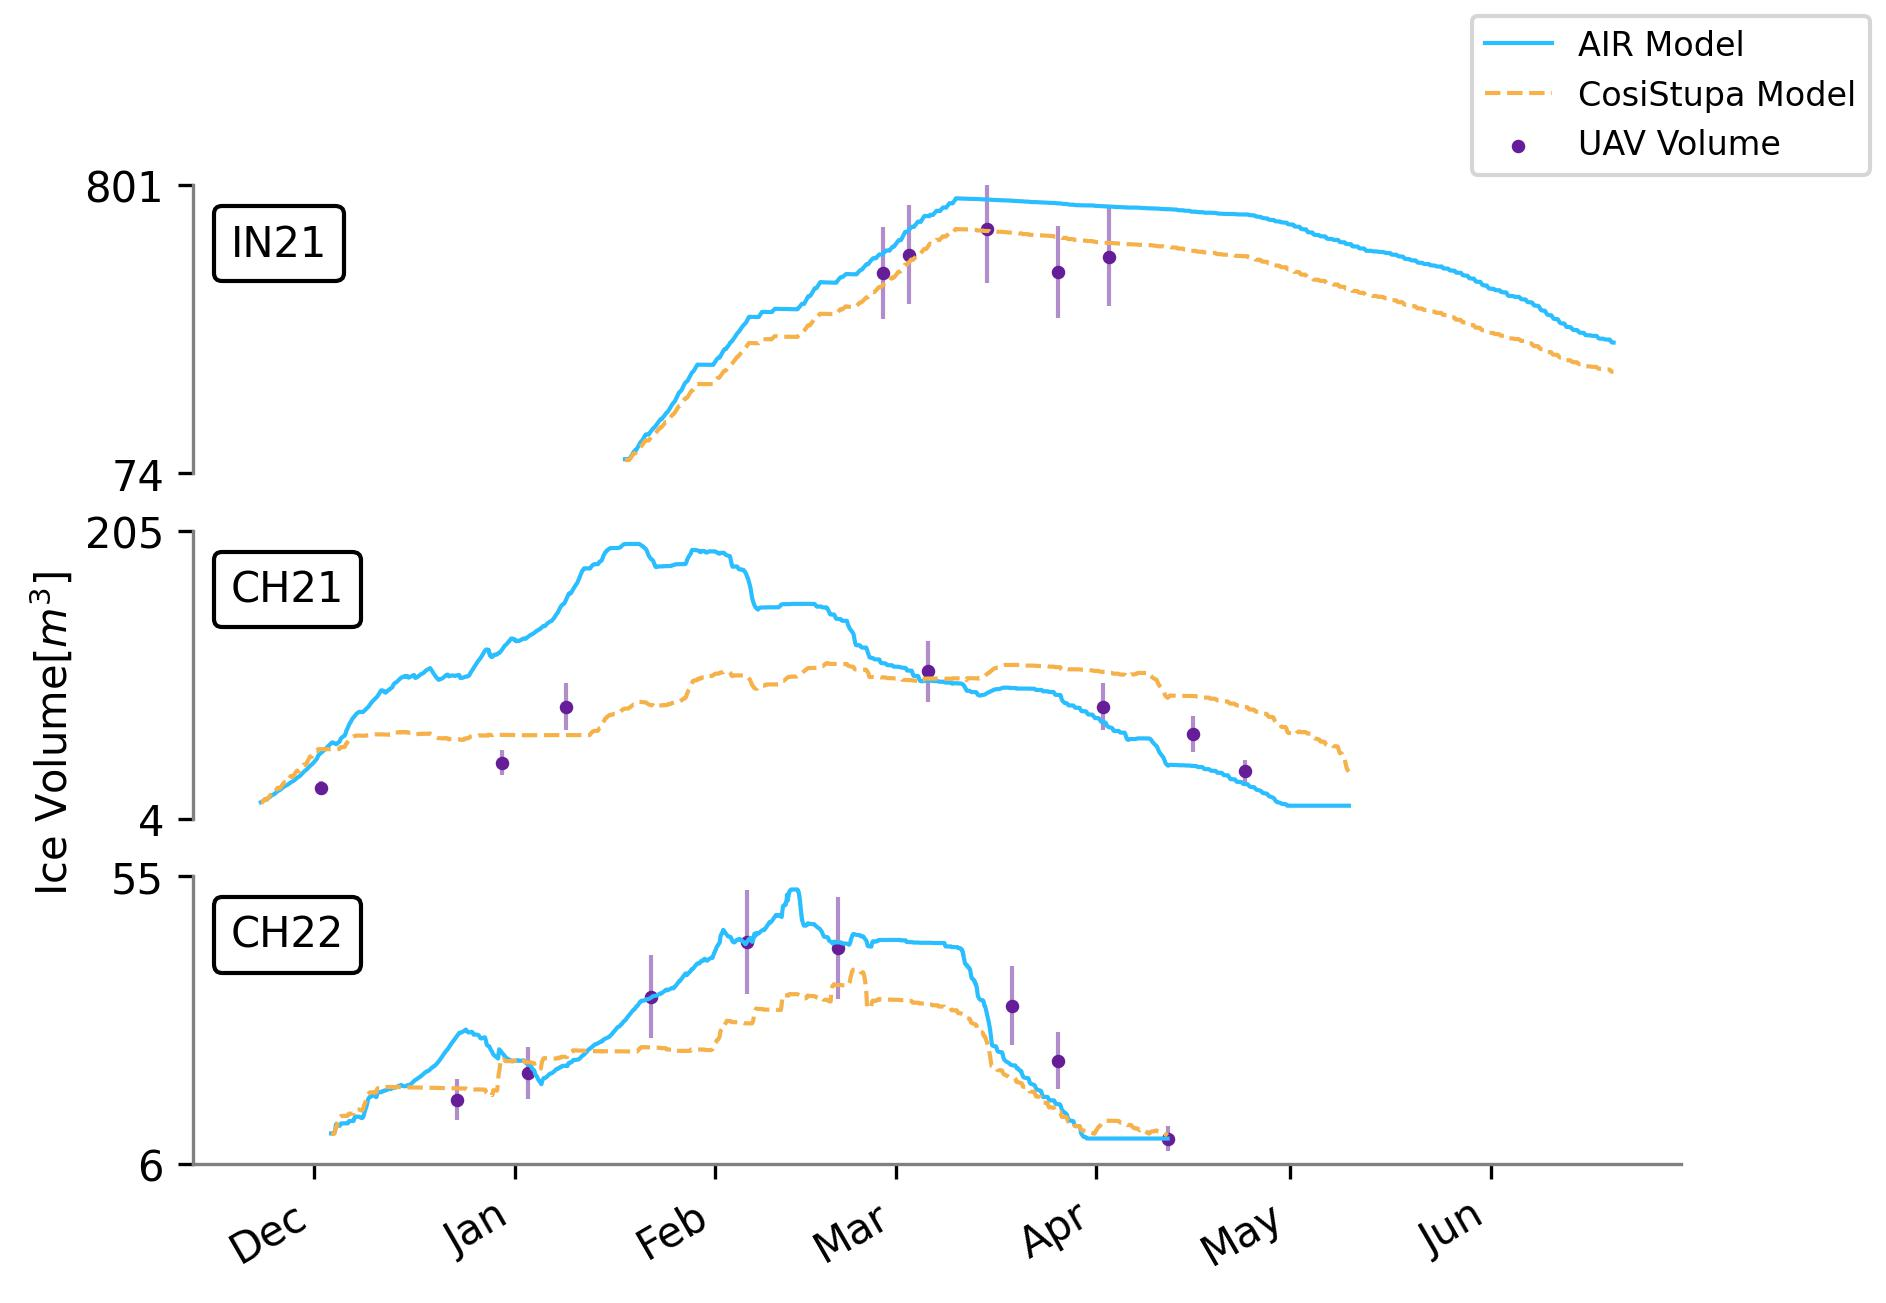
\includegraphics[width=12cm]{figs/model_compare.jpg}

\caption{Comparison of volume estimates generated from the AIR and COSISTUPA models.}

\label{fig:Cosistupa}
\end{figure}





